% !TeX spellcheck = en_US
\documentclass[12pt, a4paper]{book}
\usepackage[utf8]{inputenc}
\usepackage[english,vietnamese]{babel}

\setlength{\belowcaptionskip}{-10pt}
\setlength{\intextsep}{10pt plus 2pt minus 2pt}
\setlength{\parskip}{0.5\baselineskip}%
\setlength{\parindent}{0pt}%
% Set the title of the current document to be produced.
\newcommand{\doctitle}{{{\Huge \textbf{Data Mesh Architecture}}}}
% Command for the due date of the homework.
%\newcommand{\duedate}{\color{rltred}{\faCalendarCheckO { }Due date: May 1st, before midnight \faCalendarCheckO	}}

%------------------------------------------------------------
% Import commands for both teacher and course information.  | 
% NOTE: Change your teacher and course info in these files. |
%------>------>------>------>------>------>------>------>-->|
%-------------------------------------------------
% Teacher-specific commands                      |
%---------------                                 |
%-> Instructions: change your teacher info here. |
%------->------>------>------>------>------>---->|
%
\newcommand{\instructor}{Thanh C. Nguyen}
\newcommand{\office}{Office number}
\newcommand{\hours}{By appointment}
\newcommand{\phone}{0}
\newcommand{\college}{\textbf{Viettel Group - Viettel Digital Talent Program}}
\newcommand{\email}{thanhnc221@viettel.com.vn}
\newcommand{\faculty}{Viettel Group}
\newcommand{\department}{Information Technology Division}
                              %|
%-------------------------------------------------
% Course-specific commands                       |
%---------------                                 |
%-> Instructions: change your course info here.  |
%------->------>------>------>------>------>---->|
%
\newcommand{\semester}{2022.2}
\newcommand{\csection}{00001 \& 00002}
\newcommand{\ponderation}{2-4-3 (Theory-Lab-Homework)}
\newcommand{\coursetitle}{Data Mesh Architecture}
\newcommand{\coursenumber}{\textbf{VDT2023-SDE}}
\newcommand{\prerequisite}{All porgram courses semesters 1-4}
                               %|   
%
%------------------------------------------------------------
%-- Import packages and custom command definitons.          |
%------>------>------>------>------>------>------>------>-->|
%----------------------------------------------------
% The following is a list of LaTeX packages imports |
%------->------>------>------>------>------>---->---|
%

% The margins at the bottom of the page has been reduced.
% this allows for a slim footer.
\usepackage[left=2cm,right=2cm,top=2cm,bottom=2cm]{geometry}
% Original size:
%\usepackage[inner=1.5cm,outer=1.5cm,top=1.5cm,bottom=.5cm,margin=1in]{geometry}
\usepackage[
    colorlinks,
    %pagebackref,
    pdfusetitle,
    urlcolor=blue,
    citecolor=blue,
    linkcolor=blue,    
    plainpages=false]
{hyperref}            
% ftp://ftp.dante.de/tex-archive/fonts/bbding/bbding.pdf
%https://ctan.math.illinois.edu/fonts/bbding/bbding.pdf
\usepackage{fancyhdr, lastpage, bbding, pmboxdraw}
\usepackage{fancyvrb}
\usepackage{bigints}
\PassOptionsToPackage{usenames,dvipsnames}{xcolor}
\usepackage{graphicx,wrapfig,lipsum}
\usepackage{acronym}
\usepackage{amsthm}
\usepackage{amssymb}
\usepackage{amsmath}
\usepackage{caption}
\usepackage{xcolor}
\usepackage{bigints}
\usepackage{enumitem}
\usepackage{tabularx}
\usepackage{xltabular}
\usepackage{hyphenat}
\newcommand{\HY}{\hyphenpenalty=10000\exhyphenpenalty=10000}
\newcolumntype{b}{X}
\newcolumntype{m}{>{\HY\hsize=.3\hsize}X}
\newcolumntype{s}{>{\HY\hsize=.3\hsize}X}
\usepackage{multirow}
\usepackage{multicol}
\usepackage{makecell}
\usepackage{sectsty}
\usepackage{ragged2e}
\usepackage{framed}
%\usepackage{cite}
\sectionfont{\raggedright}
\subsectionfont{\raggedright}
\subsubsectionfont{\raggedright}
%\normalfont{\raggedright}
% pifont package doc at: https://ctan.math.ca/tex-archive/macros/latex/required/psnfss/psnfss2e.pdf
% pifont is used to define custom list and style list items using the \ding command. 
\usepackage{pifont} 
% bclogo used for making a colored box for notes. 
% @see: https://ctan.org/pkg/bclogo?lang=en
\usepackage[tikz]{bclogo} 
\usepackage{titlesec}  
\usepackage[open,openlevel=1]{bookmark}

%-- @see http://ctan.sharelatex.com/tex-archive/fonts/fontawesome/doc/fontawesome.pdf
% Font Awesome  http://ctan.math.washington.edu/tex-archive/fonts/fontawesome5/doc/fontawesome5.pdf
% https://muug.ca/mirror/ctan/fonts/fontawesome5/doc/fontawesome5.pdf
\usepackage{fontawesome5}
%---------------------------------
% ==== Font setup.
% Load any of the following fonts.
%---------------------------------
%\usepackage{lmodern}
%\usepackage{mathptmx}
%\usepackage{times}
\usepackage{mathpazo} % Palatino font.
%\linespread{1.05} % Palatino needs more leading (space between lines)
%\usepackage{tgbonum} % For Bonum/Bookman font.
\usepackage[utf8]{inputenc}
\usepackage[T1]{fontenc}
\usepackage{listings}
%---------------------------------
\usepackage{booktabs} 

\pagestyle{empty}
\usepackage{graphicx}
\usepackage{blindtext}  
\usepackage{vhistory} % for making a table for the revision history.

%------------------ Code listing
\usepackage{listings} %For code in appendix
\lstset
{ %Formatting for code in appendix
	%language=Python,
	basicstyle=\small,
	numbers=left,
	stepnumber=1,
	showstringspaces=false,
	tabsize=1,
	breaklines=true,
	breakatwhitespace=false,
	frame=leftline
}
\usepackage{algpseudocode}

%-------------------

\usepackage[Lenny]{fncychap}
\ChTitleVar{\Huge\scshape\bfseries}
\ChNameVar{\Large\bfseries}
\ChNumVar{\fontsize{60}{62}\bfseries}
%Options: Sonny, Lenny, Glenn, Conny, Rejne, Bjarne, Bjornstru

\titleformat{\section}
{\normalfont\Large\scshape}{\thesection}{1em}{}[{\titlerule[1pt]}]

%\titleformat{\part}
%[display]
%{\centering\normalfont\Large}
%{\titlerule[3pt]\vspace{3pt}\titlerule[1pt]\vspace{3pt}\Uppercase{\partname} \thepart}
%{0pt}
%{\titlerule[1pt]\vspace{3pt}\titlerule[3pt]\vspace{4pc}\bfseries\huge\scshape}

%\titleformat{\part}[frame]
%{\normalfont\Large}
%{\filright
%	\vspace{1cm}
%	\enspace \bfseries  Part \thepart \enspace
%	\vspace{1cm}
%}
%{8pt}
%{\huge\bfseries\filcenter\scshape}
%\titlespacing*{\part}{0pt}{0pt}{20pt}

\titleformat{\part}[display]
{\bfseries\huge\scshape}
{\centering Part \thepart}
{4ex}
{\titlerule
	\vspace{2ex}%
	\centering}
[\vspace{2ex}%
\titlerule \vspace{3cm} \small\normalfont\itshape ($\bullet$'v'$\bullet$) \quad CLASS = Come Late And Start Sleeping \quad ($\bullet$'v'$\bullet$)]
                                  %|  
%--------------------------------------------------------
%--> \customhrule: makes a customized rule whose width  | 
%                  should be passed as parameter.       |
%--------------------------------------------------------
\newcommand{\customhrule}[1]{
	\rule[1.4pt]{\linewidth}{#1}
}
%------------------------------------------------------
%--> \doublerule: makes a double rule.                |
%------------------------------------------------------ 
\newcommand{\doublerule}[1][.4pt]{
	\noindent
	\makebox[0pt][l]{\rule[.7ex]{\linewidth}{#1}}%
	\rule[1pt]{\linewidth}{#1}\par} 
%===== Custom Ruler commands  ==================
\renewcommand{\headrulewidth}{0.5pt}
\renewcommand{\footrulewidth}{0.5pt}

% Disable spaces between list items in a labeled list.
\setlist{noitemsep}
 
%-------------------------------------------------------------
%= The followig are declaraions of custom Lists              =
%-------------------------------------------------------------
%
%======= Green rectangles list =======================
% \Rectangle from bbind
\newlist{greenrectangles}{itemize}{4}
%\setlist[greenrectangles]{topsep=4pt,partopsep=0pt,itemsep=3pt,parsep=0pt,labelindent=0.5cm,leftmargin=*}
\setlist[greenrectangles]{itemsep=5pt,parsep=0pt,topsep=4pt,partopsep=3pt}
\setlist[greenrectangles,1]{font=\color{darkred},label={\color{darkgreen}{\Rectangle}}}

%======= Alphabetical  list =======================
\newlist{alphalist}{enumerate}{9}
\setlist[alphalist]{topsep=4pt,partopsep=0pt,itemsep=3pt,parsep=0pt,labelindent=0.5cm,leftmargin=*}
\setlist[alphalist,1]{label=(\alph*)}
%======= Non-numbered list =======================
\newlist{itemizedlist}{itemize}{9}
\setlist[itemizedlist]{topsep=4pt,partopsep=0pt,itemsep=3pt,parsep=0pt,labelindent=0.5cm,leftmargin=*}
%\setlist[itemizedlist,1 ]{label=\textbf{\alph*)}}

%======= Arrowed list =======================
\newlist{arrows}{itemize}{4}
\setlist[arrows]{topsep=4pt,partopsep=0pt,itemsep=3pt,parsep=0pt,labelindent=0.5cm,leftmargin=*}
\setlist[arrows,1]{font=\color{darkred},label={\HandRight}}

%======= Bordered square list =======================
% Colorize the selected symbol? 
% ❏
\newlist{borderedsquare}{itemize}{4}
\setlist[borderedsquare]{topsep=4pt,partopsep=0pt,itemsep=3pt,parsep=0pt,labelindent=0.5cm,leftmargin=*}
\setlist[borderedsquare,1]{label=\ding{111}}

%======= Filled, curved arrow list =======================
\newlist{curveddarrow}{itemize}{4}
\setlist[curveddarrow]{topsep=4pt,partopsep=0pt,itemsep=3pt,parsep=0pt,labelindent=0.5cm,leftmargin=*}
\setlist[curveddarrow,1]{label=\small\faMarker}

%======= Colored pen list ======================= 
\newlist{coloredPen}{itemize}{4}
\setlist[coloredPen]{topsep=4pt,partopsep=0pt,itemsep=3pt,parsep=0pt,labelindent=0.5cm,leftmargin=*}
\setlist[coloredPen,1]{font=\color{darkblue},label=\small\faMarker}

%======= Objectives list ======================= 
% ➠
\newlist{objectives}{itemize}{4}
\setlist[objectives]{topsep=4pt,partopsep=0pt,itemsep=3pt,parsep=0pt,labelindent=0.5cm,leftmargin=*}
\setlist[objectives,1]{label=\small\ding{224}}

%======= Dark starred list ======================= 
% ✸
\newlist{filledstarlist}{itemize}{4}
\setlist[filledstarlist]{topsep=4pt,partopsep=0pt,itemsep=3pt,parsep=0pt,labelindent=0.5cm,leftmargin=*}
\setlist[filledstarlist,1]{label=\small\ding{88}}

%======= Dark-bordered empty circle list ======================= 
% ❍
\newlist{emptyCircleList}{itemize}{4}
\setlist[emptyCircleList]{topsep=4pt,partopsep=0pt,itemsep=3pt,parsep=0pt,labelindent=0.5cm,leftmargin=*}
\setlist[emptyCircleList,1]{label=\small\ding{109}}

%======= Filled right arrow list ======================= 
% ➤
\newlist{filledRightArrowList}{itemize}{4}
\setlist[filledRightArrowList]{topsep=4pt,partopsep=0pt,itemsep=3pt,parsep=0pt,labelindent=0.5cm,leftmargin=*}
\setlist[filledRightArrowList,1]{label=\small\ding{228}}

%======= Numbered list: non-filled circle list ======================= 
% ➀
\newlist{numberedEmptyList}{itemize}{9}
\setlist[numberedEmptyList]{topsep=4pt,partopsep=0pt,itemsep=3pt,parsep=0pt,labelindent=0.5cm,leftmargin=*}
\setlist[numberedEmptyList,9]{label=\ding{182}}

%======= Right hand pointing list =======================
\newlist{rightHandPointingList}{itemize}{4}
\setlist[rightHandPointingList]{topsep=4pt,partopsep=0pt,itemsep=3pt,parsep=0pt,labelindent=0.5cm,leftmargin=*}
\setlist[rightHandPointingList,1]{font=\color{darkred},label={\HandRight}}

%----------------------------------------------------------------------
%=   The followig are custom colors declaraions                       |
%--  more colors codes can be found at: http://latexcolor.com/        | 
%-- usage: {\color{declared-color} some text}.                        |    
%  e.g.,: {\color{darkblue}{ This text will appear darkblue-colored}} |
%----------------------------------------------------------------------
\definecolor{darkblue}{rgb}{0,0,.6}
\definecolor{darkred}{rgb}{.7,0,0}
\definecolor{darkgreen}{rgb}{0,.6,0}
\definecolor{darkestred}{rgb}{.8,.1,0}
\definecolor{red}{rgb}{.98,0,0}
\definecolor{OliveGreen}{cmyk}{0.64,0,0.95,0.40}
\definecolor{CadetBlue}{cmyk}{0.62,0.57,0.23,0}
\definecolor{lightlightgray}{gray}{0.93}
\definecolor{vanierred}{RGB}{210,0,2}
\definecolor{darkestblue}{rgb}{0.0, 0.0, 0.55}
\definecolor{darkblue}{rgb}{0,0,.6}
\definecolor{darkred}{rgb}{.7,0,0}
\definecolor{darkgreen}{rgb}{0,.6,0}
\definecolor{darkestred}{rgb}{.8,.1,0}
\definecolor{red}{rgb}{.98,0,0}
\definecolor{OliveGreen}{cmyk}{0.64,0,0.95,0.40}
\definecolor{CadetBlue}{cmyk}{0.62,0.57,0.23,0}
\definecolor{lightlightgray}{gray}{0.93}
\definecolor{darkorange}{rgb}{255,140,0}
\definecolor{fluorescentyellow}{rgb}{0.8, 1.0, 0.0}
\definecolor{darkyellow}{rgb}{1,1,0.34}
\definecolor{lightyellow}{rgb}{1,1,0.6}
\definecolor{coolblack}{rgb}{0.0, 0.18, 0.39}
\definecolor{lightgray}{rgb}{.9,.9,.9}
\definecolor{darkgray}{rgb}{.4,.4,.4}
\definecolor{purple}{rgb}{0.65, 0.12, 0.82}
\definecolor{gray}{rgb}{0.4,0.4,0.4}
\definecolor{cyan}{rgb}{0.0,0.6,0.6}
\definecolor{dkgreen}{rgb}{0,0.6,0}
\definecolor{gray}{rgb}{0.5,0.5,0.5}
\definecolor{mauve}{rgb}{0.58,0,0.82}
\definecolor{lightblue}{rgb}{0.0,0.0,0.9}
\colorlet{punct}{red!60!black}
\definecolor{background}{HTML}{EEEEEE}
\definecolor{delim}{RGB}{20,105,176}
\colorlet{numb}{magenta!60!black}
\definecolor{coolblack}{rgb}{0.0, 0.18, 0.39}
\definecolor{forestgreen}{rgb}{0.0, 0.27, 0.13}
\definecolor{firebrick}{rgb}{0.7, 0.13, 0.13}
\definecolor{rltred}{rgb}{0.75,0,0}
\definecolor{rltgreen}{rgb}{0,0.5,0}
\definecolor{rltblue}{rgb}{0,0,0.75}
\definecolor{indigo}{rgb}{0.0, 0.25, 0.42}
\definecolor{jazzberryjam}{rgb}{0.65, 0.04, 0.37}
\definecolor{lava}{rgb}{0.81, 0.06, 0.13}
\definecolor{royalblue}{rgb}{0.0, 0.14, 0.4}
\definecolor{prussianblue}{rgb}{0.0, 0.19, 0.33}
\definecolor{prune}{rgb}{0.44, 0.11, 0.11}
\definecolor{cerisepink}{rgb}{0.93, 0.23, 0.51}
\definecolor{oxfordblue}{rgb}{0.0, 0.13, 0.28}
\definecolor{crimsonglory}{rgb}{0.75, 0.0, 0.2}
\definecolor{fireenginered}{rgb}{0.81, 0.09, 0.13}

%============================
% Commands for inserting colored text.
\newcommand{\bluetext}[1]{\textcolor{darkblue}{#1}}
\newcommand{\redtext}[1]{\textcolor{jazzberryjam}{#1}}

%=================================================================================================
% Command for styling tabled row header (left, center or right)
% Usage example: \thead{<Header text 1>} & \thead{<Header 2>} & \thead{<Header 3>} & \thead{<Header 4>} 
%\newcommand*{\thead}[1]{\multicolumn{1}{l}{\bfseries #1}}	

%--------------------------------------------------
% ==== Doc header and footer setup.               |
%-------------------------------------------------- 
\fancypagestyle{plain}{%
	\fancyhf{}%
	\fancyhead[LE, RO]{\small{\textbf{\leftmark}}}
	%\fancyhead[RE,RO]{\small{\textbf{Theory Summary}}}
	\fancyfoot[RO, LE] {{\small{\thepage}}}
	\fancyfoot[LO, RE]{{\small{Mini-project Report - \textbf{Data Mesh Architecture}} }}
	\renewcommand{\headrulewidth}{0.5pt}% Line at the header invisible
	\renewcommand{\footrulewidth}{0.5pt}% Line at the footer visible
}



\renewcommand{\thefootnote}{\arabic{footnote}}
\pagestyle{plain}
\fancyhf{}
%- Disable the horizontal ruler in the header section.
\renewcommand{\headrulewidth}{0.5pt}
\renewcommand{\footrulewidth}{0.5pt}
%\rfoot{{Page \thepage\ of \pageref{LastPage}}}
%\cfoot{{\small{\college { } - { } \semester} }}
%\lfoot{{\small{Ta Ngoc Minh - CTTT Data Science \& AI 01 - K66} }}
%- TODO: move the header content here.
%\fancyhead[LE,LO]{\small{\textbf{Introduction to Artificial Intelligence}}}
\fancyhead[LE, RO]{\small{\textbf{\rightmark}}}
\fancyfoot[RO, LE] {{\small{\thepage}}}
\fancyfoot[LO, RE]{{\small{Mini-project Report - \textbf{Data Mesh Architecture}} }}
\thispagestyle{plain}
%------------------------------------------------------------

\newcolumntype{L}[1]{>{\raggedright\arraybackslash}p{#1}}
\newcolumntype{C}[1]{>{\centering\arraybackslash}p{#1}}
\newcolumntype{R}[1]{>{\raggedleft\arraybackslash}p{#1}}

%-- Spacing commands ------ 
\newcommand{\vspbpara}{\vspace*{.09in}}    
\newcommand{\customvspace}{\vspace{.5cm}}    
\titlespacing{\section}{0pt}{12pt}{9pt}
%-----
\newcommand{\vtitlespacing}{\vskip 0.3cm}
\newcommand{\paragraphentry}[1]{\noindent \textbf{\Large \underline{#1}} }
   
%
%---> Genereate & inject metadata describing                |
%     the produced document                                 |
%--------------------------------------------------------------
%-- Set up the hyperref package.                              |
%-- Generate and inject metadate in the produced PDF document |
%------>------>------>------>------>------>------>------>-->---
 \hypersetup{pdfauthor={Ta Ngoc Minh},%
    pdftitle={\coursenumber -- \coursetitle},%
    pdfsubject={\doctitle},%
    pdfkeywords={\college,  \department},%
    pdfproducer={LaTeX},%
    pdfcreator={pdfLaTeX},
    bookmarks,
    bookmarksnumbered = true,
    bookmarksopen     = true,
    pdfpagelabels     = true,
    pdfstartview={FitH null null 1.0}
}                                  %|
%------------------------------------------------------------


%-----------------------------------------------------------
% Uncomment the following if you want to insert a watermark! 
%
%--> Watermark package settings: 
%\usepackage{draftwatermark}
%\SetWatermarkText{DRAFT}
%\SetWatermarkScale{0.5}
%\SetWatermarkColor[gray]{0.8}
%-------------------------------------------------
\hypersetup{hidelinks}
\begin{document} 
	
    \raggedbottom
    \clearpage
    \pagenumbering{roman}
    \thispagestyle{empty}
    %-------------------------------------------------------------
    %-- Make the header of the document                          |
    %------>------>------>------>------>------>------>------>--> |
    %--------------------------------------------------------------------------
%- The following produces the document header including the title.        |
%- The document header includes: the college/university name, faculty,    |
%  department, course number and title as well as the assignment/homework | 
%  title and due date.                                                    | 
%-------------------------------------------------------------------------|
%
\noindent % <-- need to have this first.
%
\begin{minipage}{.7\textwidth}
    { \textsc{\textbf{Viettel Group - Viettel Digital Talent Program}}}{ }\\ 
    \small\textsc{Viettel Digital Talent Residency 2023}\\%
    \small\textsc{Software \& Data Engineering Sector}
\end{minipage}%
\hfill	
\begin{minipage}{0.3\textwidth}%
    \raggedleft%
    {\Large \textsc{\textbf{Period 1}} \par}
    \doublerule % insert a double rule.
    \textsc{Mini-project Report}\\
\end{minipage}%
\vskip 5pt
\hrule \vskip 2pt \hrule
\vspace{1.8cm}
{
    %--> Insert homework title and due date.
    \begin{center}
    	
\includegraphics[scale=0.4]{Viettel.png}
    \end{center}
	\vspace{1.8cm}
    \hrule \vskip 2pt \hrule
    \vspace{1cm}
    \centering
    {\scshape 
        \Huge \color{darkestred}{\doctitle}{ }
    \vspace{1cm}    
}
{
    \hrule \vskip 2pt \hrule \vspace{1cm}
    
    \centering  \textsc{\textbf{\Large Mini-project Report - Topic 8}} \\
    \vspace{.4cm}
    \textsc{Data Engineering Specialization} \\
    \vspace{.5cm}\vskip 20pt
    \selectlanguage{vietnamese}
    \small{\textbf{\normalsize \textsc{Resident:} Tạ Ngọc Minh}\\
    BSc. student in Data Science \& AI @ HUST
    	\vskip 5pt
	\vskip 20pt
	\textbf{\normalsize \textsc{Supervisor:} Mr. Nguyễn Chí Thanh}
    \vspace{.5cm}
    \selectlanguage{english}
}    
\vspace{.5cm}
\hrule
\vskip 5cm
\textbf{Hanoi - 2023}

    \selectlanguage{english}
    %\hrule width0.3\textwidth
    \begingroup
    \normalsize
\chapter*{Preface}
\addcontentsline{toc}{chapter}{Preface}
\justifying
\selectlanguage{vietnamese}
Dear the board of directors of Viettel Group, the mentors, and all of my friends,

This document is a part of my research mini-project as a data engineer intern for the first period of Viettel Digital Talent 2023 Program. The completion of this research report does not mean the end of my duties as learners. In fact, this report is a first step towards consistently studying what I have reviewed and written here.

Data has grown up so quickly recently. The term 'big data' has become familiar with every tech-lovers is the clearest evidence of the explosion of data. This leads to many requirements of upgrading the current system and management, along with finding new architecture to store, process and analyze data. Once the central data lake has been overloaded, we need to design a decentralized architecture. This report is written under the research about the Data Mesh architecture, a new design that was first defined by Zhamak Dehghani in 2019.

To write this document, I would like to give many thanks to Viettel Group, and Viettel Digital Talent program for giving me chance to do my research. I want to send a big thanks to Mr. Nguyễn Chí Thanh, and all the mentors of the first period of the program, who gave me many useful lectures and guidance. Also, I want to say thanks to professor Huỳnh Thị Thanh Bình, professor Đỗ Tuấn Anh for their initial supports, and many other professors at the International Research Center for AI and the School of Information and Communication Technology, Hanoi University of Science and Technology about their public documents about data engineering. Last, I would like to say thanks to all of my friends, who always read my documents, comment about them and support me whenever I need.

Because this document is written in such a short time and some of the concepts are so new and hard to understand for a fresher like me, it is so hard to make sure it is completely correct, including the grammar errors and formatting errors in \LaTeX. I would love to receive your contributions via \underline{\textbf{\href{mailto:ngocminhta.nmt@gmail.com}{ngocminhta.nmt@gmail.com}}}.

Thank you for reading this report and looking forward to getting many comments from you.\\
\vspace{0.5cm}

\raggedleft
\textbf{Ngoc-Minh Ta}\\
\textit{Viettel Digital Talent Residency 2023}

\justifying
\selectlanguage{english}

        \tableofcontents
        \listoffigures
        \addcontentsline{toc}{chapter}{List of Figures}
        \let\cleardoublepage\clearpage
        \listoftables
        \addcontentsline{toc}{chapter}{List of Tables}
        \let\cleardoublepage\clearpage
    \endgroup
    
    \begingroup
        \frontmatter
        \justifying
        \let\cleardoublepage\clearpage
    \endgroup
    
    \mainmatter
    \justifying
    \normalsize
%--------------------
\chapter{Problems and Initial Approach}

\section{Real-life Problem}
\subsection{A problem from history}
Many organizations have invested in building a central data lake. To make data-driven business, there is a central data administration team take the responsibility for this.

\begin{figure}[h]
	\begin{framed}
		\centering
		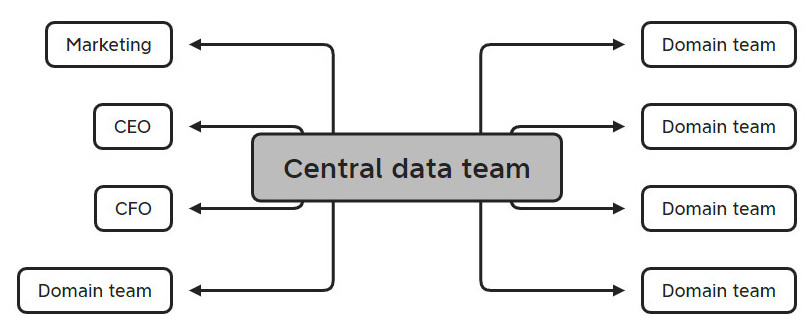
\includegraphics[width=14cm]{CentralDataTeam.jpg}
		\caption{Central data team in a data-driven business}
		\label{centraldata}
	\end{framed}
\end{figure}

This model works quite well at the first time, however, after a while, the team became overloaded with tasks and requests, leading to a decrease in competitiveness due to slow analysis. Their slow response to changes in the operational database is due to the need to fix broken data pipelines and get domain expertise. This is a daunting task. \cite{datamesh2022prologue,datameshweb}

In some firm, applying domain-driven design strategies involve independent domain teams and a decentralized micro-service architecture to relieve burden on the central data team. However, these teams must contact the overloaded central data team to obtain essential data-driven insights. \cite{datamesh2022prologue}

\subsection{Demands from recent developments}
Let's consider the scale-up of the software development over time. When one task grow bigger and bigger, we have to decentralize it into many smaller tasks, otherwise, all the organization will overload and lost of control. Take into consideration what we have done for the scale-up of software development:
	\begin{itemize}[nosep]
		\item Decentralize business into domains;
		\item Decentralize engineering into autonomous teams;
		\item Decentralize monolith into micro-services;
		\item Decentralize operations into DevOps teams.
	\end{itemize}

Hence, the next thing we need to do is scaling up data analytics by decentralizing data lake into data mesh.\cite{datameshweb}

\section{Initial approach}
\subsection{What is Data Mesh?}
The term data mesh was first stated by Zhamak Dehghani in 2019 and is based on four fundamental principles, which will be discussed in depth later:
	\begin{itemize}[nosep]
		\item Principle of Domain Ownership;
		\item Principle of Data as a Product;
		\item Principle of the Self-Serve Data Platform;
		\item Principle of Federated Computational Governance.
	\end{itemize}


\subsection{What will changes after data mesh?}
Data mesh is a fresh method for business intelligence, data analysis and management that is based on an distributed architecture. Along with that, data lake and data warehouse do not disappear, they just become nodes in the mesh. \cite{machado2022data,shiftkpmg}

\begin{figure}[h]
	\begin{framed}
		\centering
		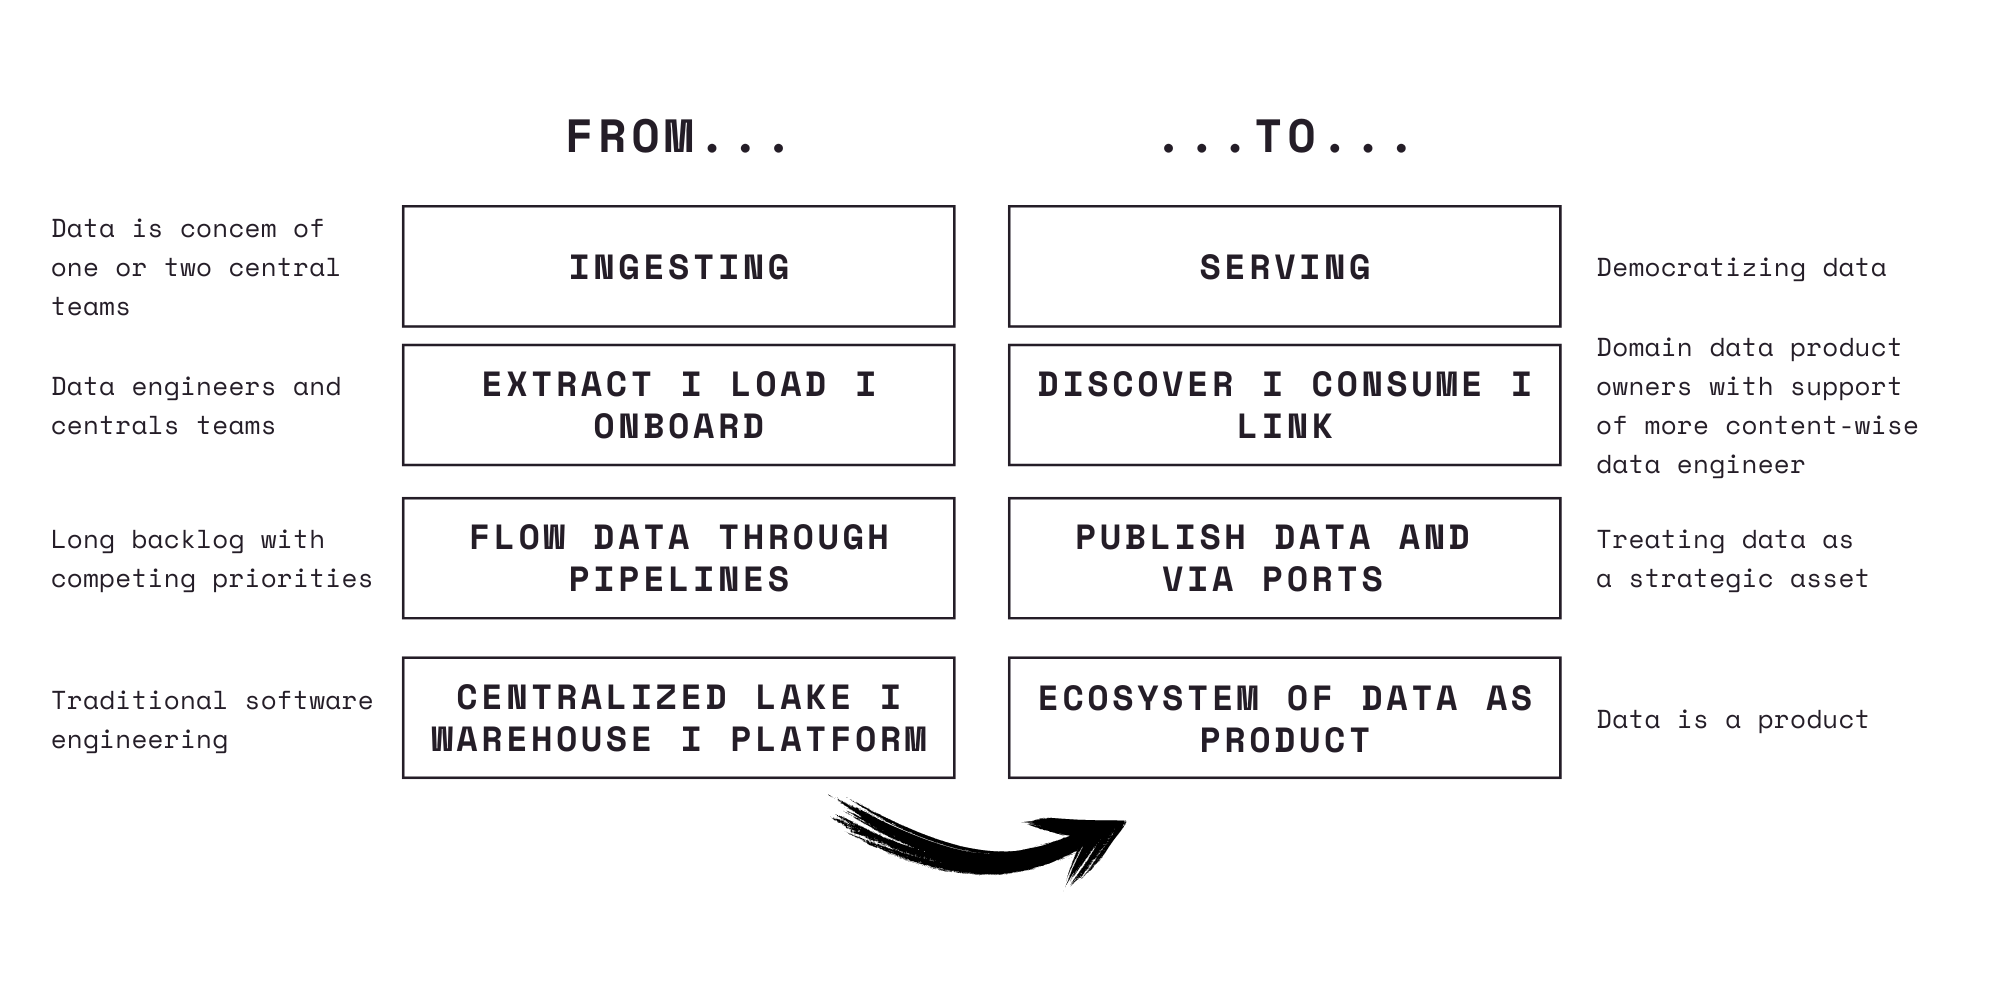
\includegraphics[width=16.5cm]{CulturalShift.png}
		\caption{Cultural shift after implementing data mesh}
		\label{culturalshift}
	\end{framed}
\end{figure}

Data mesh ensures organizations to continue to apply some data lake principles, and data lake tooling for internal implementation of data products, but it would not be the centerpiece anymore.

It is an implementation detail sub-serving the idea of domain data product as the first-class concern. The same applies to data warehouse in terms of business reporting and visualization \cite{shiftkpmg}. It also cause a cultural shift in the organization, also, a fundamental shift in the assumptions, architecture, technical solutions, and social structure of our organizations. \cite{datamesh2022ch1}

\begin{figure}[h]
	\vspace*{-.3cm}
	\begin{framed}
		\centering
		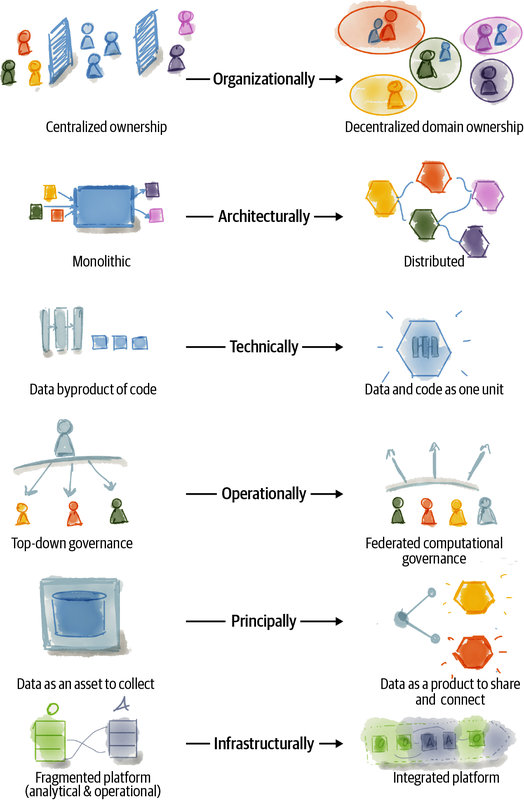
\includegraphics[width=12cm]{OrgChanges.png}
		\caption{Data mesh dimensions of organizational changes}
		\label{orgchange}
	\end{framed}
\end{figure}

In its most basic form, it can be characterized by four interacting principles, which will be discussed in depth in section \ref{4principles}.

\let\cleardoublepage\clearpage

\chapter{Data Mesh Architecture Design}
\section{Four Fundamental Principles of Data Mesh}\label{4principles}
Four simple principles can represent the logical architecture and operating model of data mesh. They are intended to move us closer to the goals of data mesh: increasing the value of data at scale, maintaining agility as an organization grows, and embracing change in a complex and turbulent business context.

\subsection{Principle of Domain Ownership}
Data mesh is a decentralized and distributed data architecture that follows the seams of organizational units, rather than technological partitions. It is founded on domain-driven design (DDD) strategies, which define a domain as “a sphere of knowledge, influence or activity.” Data mesh gives the data sharing responsibility to each of the business domains, each domain is responsible for the data it is most familiar with. DDD’s Strategic Design embraces modeling based on multiple models each contextualized to a particular domain, called a bounded context \footnote{A bounded context is the delimited applicability of a particular model that gives team members a clear and shared understanding of what has to be consistent and what can develop independently. \cite{dddevan}}. As Z. Dehghani’s recommendation, data mesh adopts the boundary of bounded contexts to individual data products - data, its models, and its ownership.

Domain data ownership is the foundation of scale in a complex system like enterprises today. When we map the data mesh to an organization and its domains, we discover a few different archetypes of domain-oriented analytical data:
	\begin{itemize}[nosep]
		\item Source-aligned domain data (native data product): Analytical data reflecting the business facts generated by the operational systems.
		\item Aggregate domain data: Analytical data that is an aggregate of multiple upstream domains.
		\item Consumer-aligned (fit-for-purpose) domain data: Analytical data transformed to fit the needs of one or multiple specific use cases.
	\end{itemize}

\begin{figure}[h]
	\begin{framed}
		\centering
		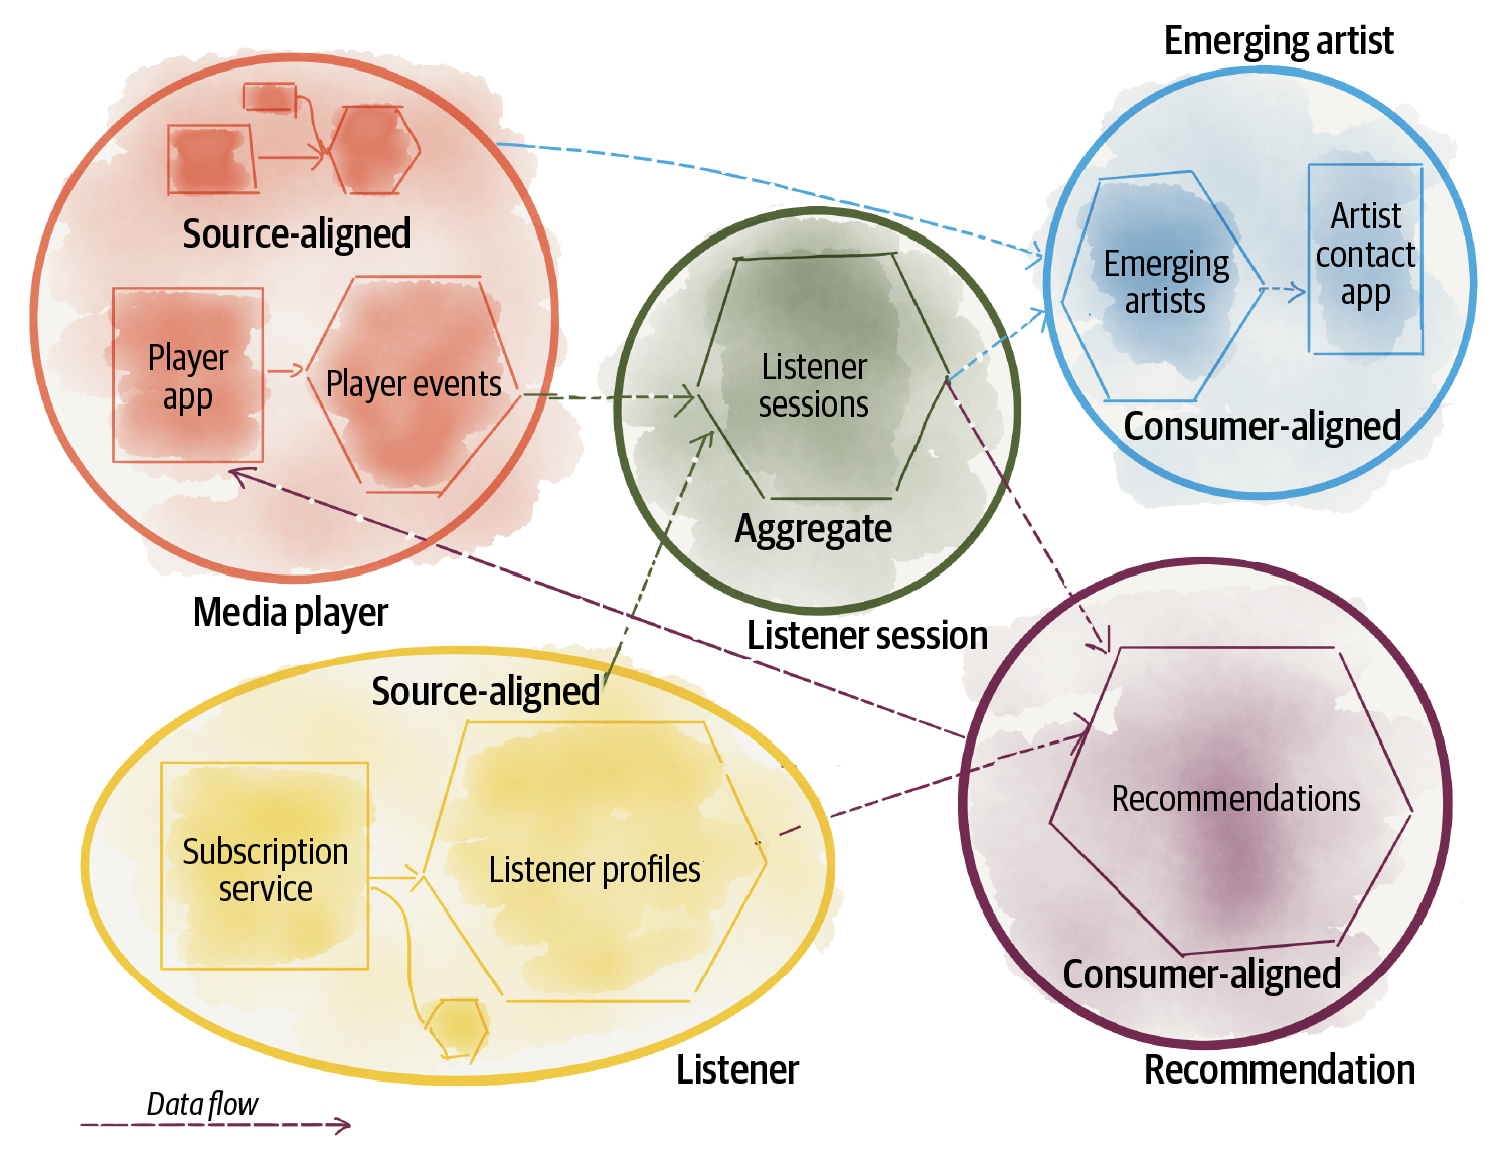
\includegraphics[width=12cm]{DecomposeData.png}
		\caption{Decomposing the analytical data ownership and architecture, aligned with business domains, along with their data archetypes.}
		\label{DecomposeData}
	\end{framed}
\end{figure}

The shift toward domain-oriented data ownership leads to accepting and working with real-world messiness of data, particularly in high-speed and scaled environments:
	\begin{itemize}[nosep]
		\item Push Data Ownership Upstream.
		\item Define Multiple Connected Models.
		\item Data mesh gives long-term domain ownership with obligation to exchange data.
		\item Hide the Data Pipelines.
	\end{itemize}

Domains are taking up extra data responsibility with data mesh. To acquire agility and authenticity, responsibility and efforts transfer from a centralized data team to domains. \cite{datamesh2022ch2}

\subsection{Principle of Data as a Product}
\begin{figure}[h]
	\begin{framed}
		\centering
		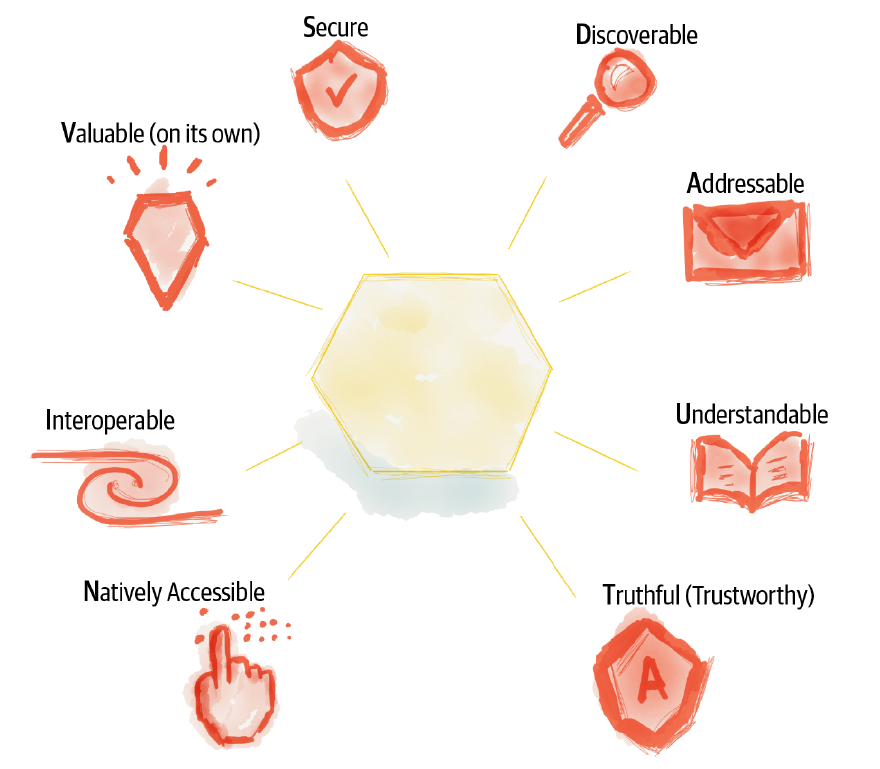
\includegraphics[width=11cm]{dautnivs.png}
		\caption{The baseline usability attributes of data products (DAUTNIVS)}
		\label{dautnivs}
	\end{framed}
\end{figure}

Data as a product is a response to data siloing and shifts data culture towards accountability and trust. It includes baseline data product usability attributes (see figure \ref{dautnivs}), which are an addition to FAIR data principles\footnote{\textbf{F}indability, \textbf{A}ccessibility,  \textbf{I}nteroperability, and \textbf{R}eusability. \cite{fair}}.

The introduction of analytical data as a product adds to the list of existing responsibilities
of cross-functional domain teams \cite{datamesh2022ch3} and expands their roles to Data product developer, and Data product owner.

Define these roles for each domain and allocate one or multiple people to the roles depending on the complexity of the domain and the number of its data products. Moreover, to make a data as a product, we need to satisfy these conditions:
	\begin{itemize}[nosep]
		\item Reframe the Nomenclature.
		\item Think of Data as a Product, not a mere asset.
		\item Establish a Trust-But-Verify Data Culture.
		\item Join Data and Compute as One Logical Unit.
	\end{itemize}

\subsection{Data contract}
Data contract is an agreement between a service provider and data consumers. It is not in-depth legal documents, but a process to help data producers and data consumers get on the same page. It refers to the management and intended usage of data between different organizations to ensure reliable and high-quality data that can be trusted by all parties involved. \cite{contract}

\begin{figure}[h]
	\begin{framed}
		\centering
		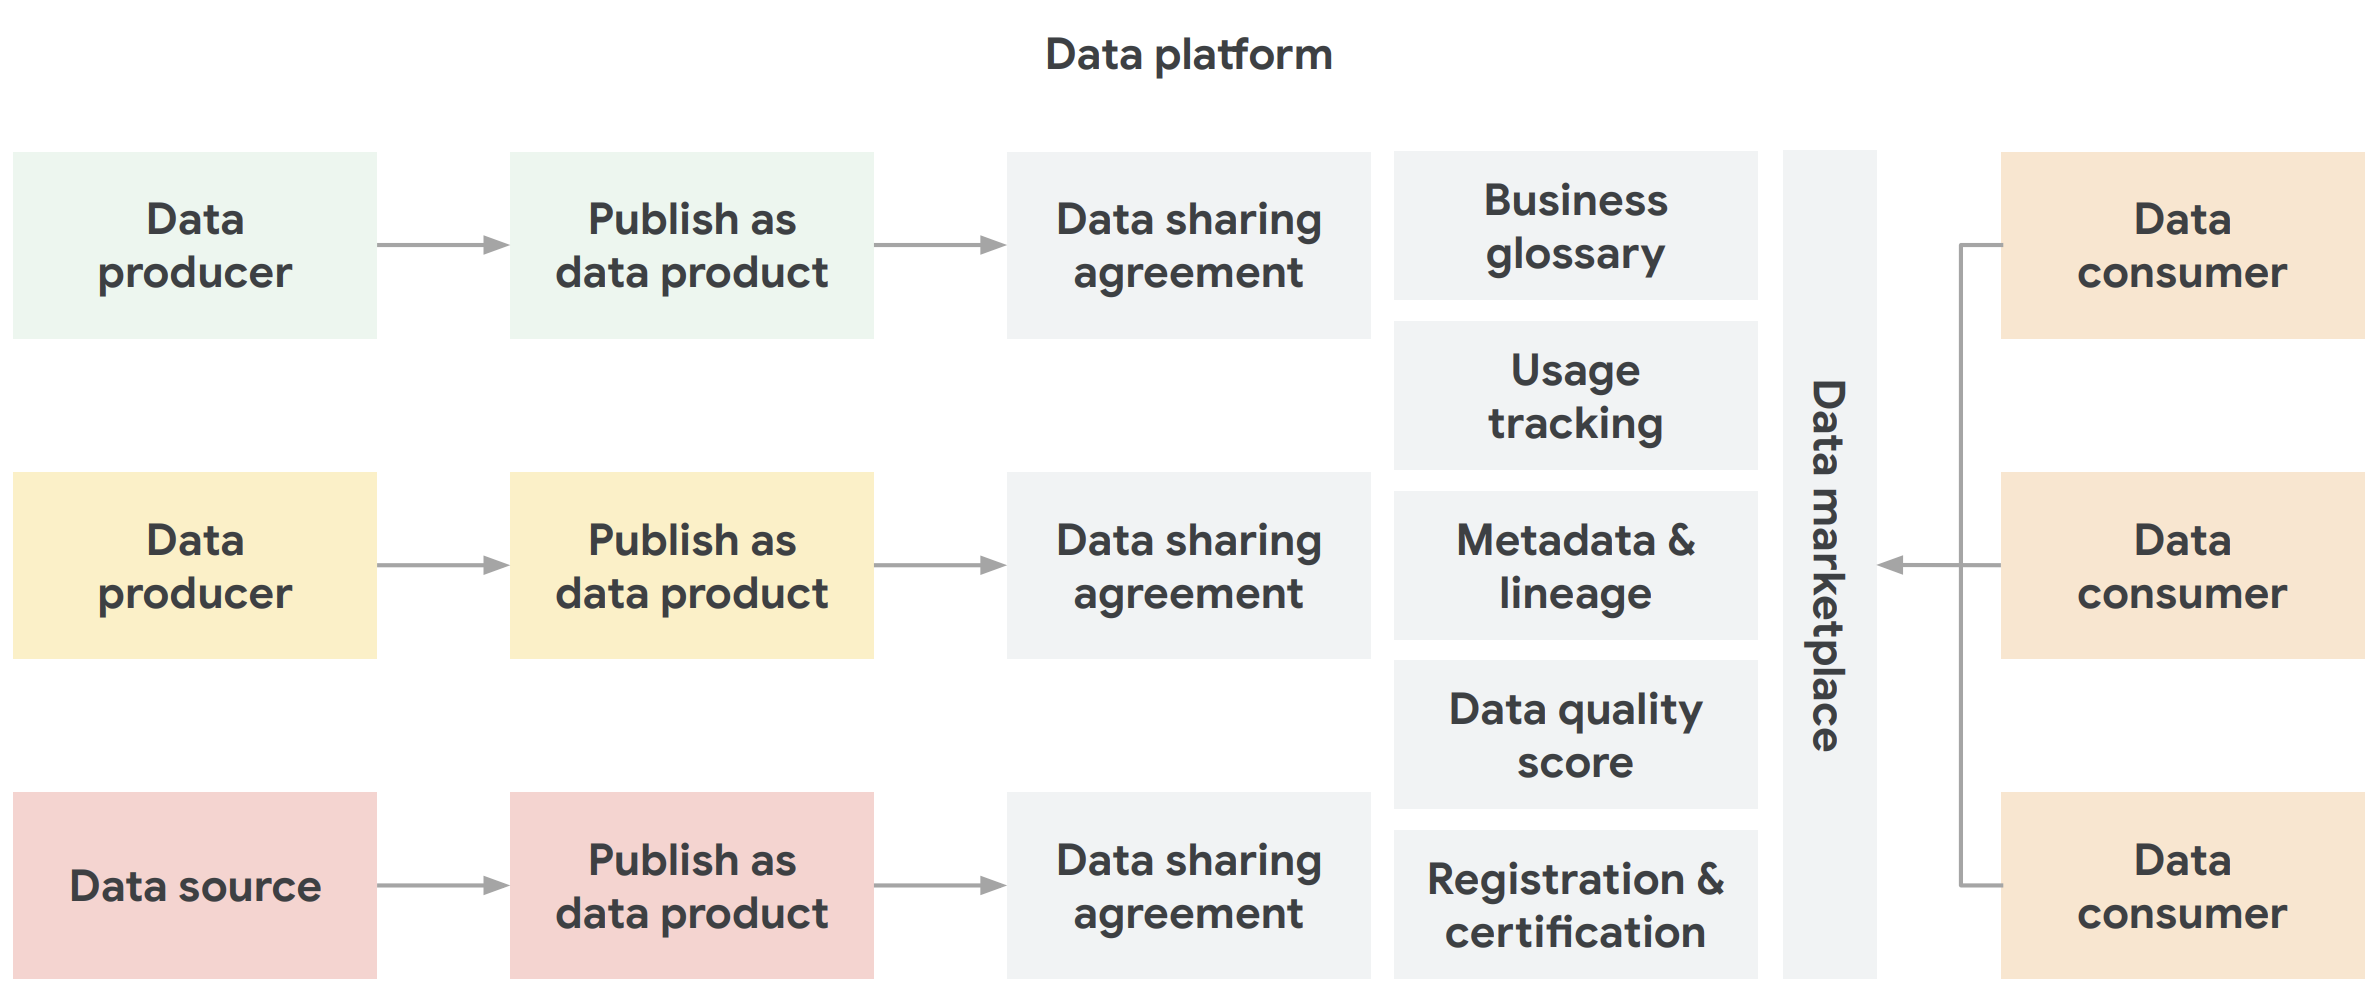
\includegraphics[width=13cm]{datacontract.png}
		\caption{Data contract in organization}
		\label{datacontract}
	\end{framed}
\end{figure}

Data contract enforces specific formats, limitations, and semantic meanings to prevent data quality difficulties when it brought into data warehouse is unusable by data consumers.

The data mesh strategy is a critical notion for ensuring that data responsibilities are dispersed across domains. Contract is the method that helps producers and consumers communicate effectively, and they are especially critical when dealing with widely spread data.

Data contracts vary depending on data and organization, there is no standardization for them, but normally, we have:
	\begin{itemize}[nosep]
		\item What data is being extracted.
		\item Type and frequency of consumption.
		\item Details of data ownership/ingestion.
		\item Levels of data access necessary.
		\item Information on security and governance (e.g., anonymization).
		\item How it affects any system(s) that intake may have an effect on.
	\end{itemize}

As organizations move towards a data mesh approach, and data is viewed as a product, organizations must create data contracts to keep data connected and running smoothly.

\subsection{Principle of the Self-Serve Data Platform}
The principle aims to empower domain teams by hiding low-level complexity behind simpler abstractions and minimizing friction from their journeys to exchanging data products as a unit of value, using decentralized, interoperable methods.


\subsection{Principle of Federated Computational Governance}
In contrast to data lake and data warehouse's governance models, data mesh one shifts to decentralized, federated computational governance.

The data mesh governance model consists of three complementary pillars:
	\begin{itemize}[nosep]
		\item \textbf{System thinking:} Manage the behavior of the mesh to create value by exchanging data products at scale.
		\item \textbf{Apply a federated operating model:} Create incentives to align domains' data products and ecosystem success.
		\item \textbf{Embed the governance policies} into each data product in an automated and computational fashion. 
	\end{itemize}

To bring these three pillars together, Figure \ref{DataGov} shows an example of this model.

\begin{figure}[h]
	\begin{framed}
		\centering
		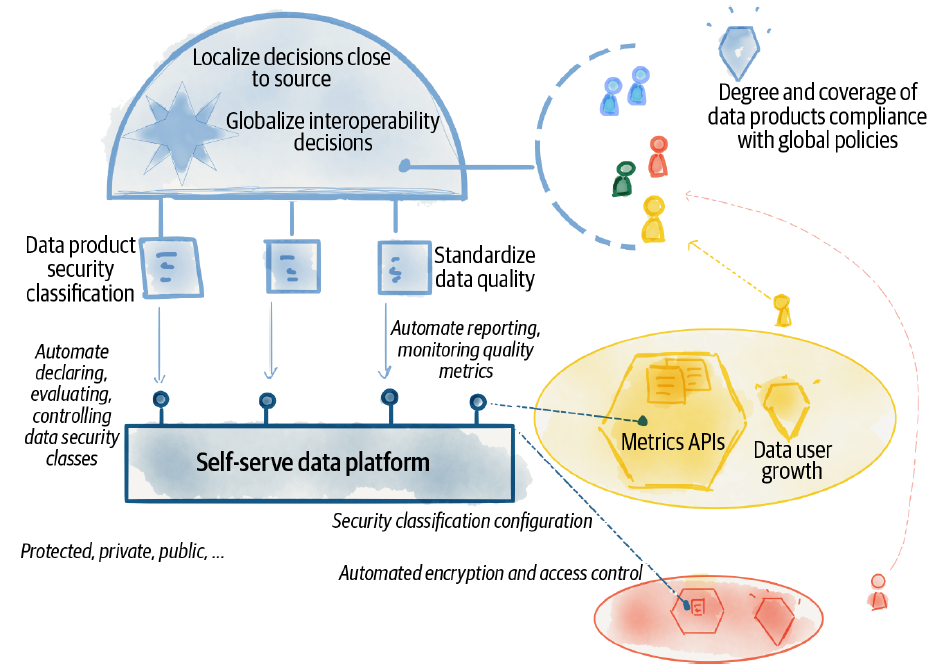
\includegraphics[width=12cm]{DataGov.png}
		\caption{Example of data mesh governance operating model}
		\label{DataGov}
	\end{framed}
\end{figure}

Data mesh governance seeks to improve existing data governance by finding the dynamic equilibrium between localization and globalization of decisions. It requires trustworthiness and useful data across multiple domains to train ML-based solutions.

\section{Why we need Data Mesh?}
Data mesh is what comes after an inflection point, shifting our approach, attitude, and technology toward data. Data mesh assumes a new default starting state: proliferation of data origins within and beyond organizations’ boundaries, on one or across multiple cloud platforms.

After the inflection point, data mesh make us reimagine data, specifically how to design solutions to manage it, how to govern it, and how to structure our teams: \cite{datamesh2022p2}
	\begin{xltabular}{\textwidth}{||s|m|b|}
		\caption{Summary of after the inflection point with data mesh} \label{tab:AfterInflection} \\
		
		\hline \multicolumn{1}{||s|}{\textbf{Goal}} & \multicolumn{1}{m|}{\textbf{What to do}} & \multicolumn{1}{b|}{\textbf{How to do it}} \\ \hline 
		\endfirsthead
		
		\multicolumn{3}{c}%
		{\tablename\ \thetable{} \textit{-- continued from previous page}} \\
		\hline \multicolumn{1}{||s|}{\textbf{Goal}} & \multicolumn{1}{m|}{\textbf{What to do}} & \multicolumn{1}{b|}{\textbf{How to do it}} \\ \hline 
		\endhead
		
		\hline \multicolumn{3}{||r|}{{\textit{continued on next page --}}} \\ \hline
		\endfoot
		
		\hline
		\endlastfoot
		
		\multirow{4}{*}{\parbox{.17\textwidth}{Manage changes to data gracefully in a complex, volatile, and uncertain business environment}} & Align business, tech, and data & Create cross-functional teams responsible for long-term data ownership.\\
		\cline{2-3}
		& Close the gap between the operational and analytical data planes  & Dumb pipes should be used to integrate applications and data products.\\ 
		\cline{2-3}
		& Localize data changes to business domains & Localize maintenance and ownership of data products in their specific domains \newline Create clear contracts between domain-oriented data products to reduce impact of change.\\
		\cline{2-3}
		& Reduce the accidental complexity of pipelines and copying of data & Break down pipelines, move transformation logic into data products.\\
		\cline{1-3}
		
		\multirow{4}{*}{\parbox{.17\textwidth}{Sustain agility in the face of growth}} & Remove centralized architectural bottlenecks & Remove centralized data warehouses and data lakes \newline Enable peer-to-peer data sharing of data products through their data interfaces.\\
		\cline{2-3}
		& Reduce the coordination of data pipelines & Decomposition of pipeline architecture from functional to domain-oriented. \newline Introduce explicit data contracts between domain-oriented data products.\\
		\cline{2-3}
		& Reduce coordination of data governance & Delegate governance responsibilities to autonomous domains and their data product owners \newline Automate governance policies as code embedded and verified by each data product quantum.\\
		\cline{2-3}
		& Enable team autonomy & Give domain teams autonomy in moving fast independently.\newline Balance team autonomy with computational standards to create global consistency.\newline Provide domain-agnostic infrastructure capabilities to empower domain teams.\\
		\cline{1-3}
		\multirow{3}{*}{\parbox{.17\textwidth}{Increase value from data over cost}} & Abstract complexity with a data platform & Create a data-developer-centric and a data-user-centric infrastructure to remove friction and hidden costs in data development and use journeys \newline Define open and standard interfaces for data products to reduce vendor integration complexity.\\
		\cline{2-3}
		& Embed product thinking everywhere & Focus and measure success based on data user and developer happiness \newline Treat both data and the data platform as a product. \\
		\cline{2-3}
		& Go beyond the boundaries of an organization & Share data across physical and logical boundaries of platforms and organizations with standard and internet-based data sharing contracts across data products.\\
	\end{xltabular}

While the evolution of data architecture has been necessary and an improvement, all of the existing analytical data architectures share a common set of characteristics that inhibit them from scaling organizationally. They are all monolithic with centralized ownership and technically partitioned. It is no longer valid when data gets sources from hundreds of microservices and millions of devices from within and outside of enterprises.

\section{Data Mesh Architecture Design}
\subsection{The Logical Architecture}
\begin{figure}[h]
	\begin{framed}
		\centering
		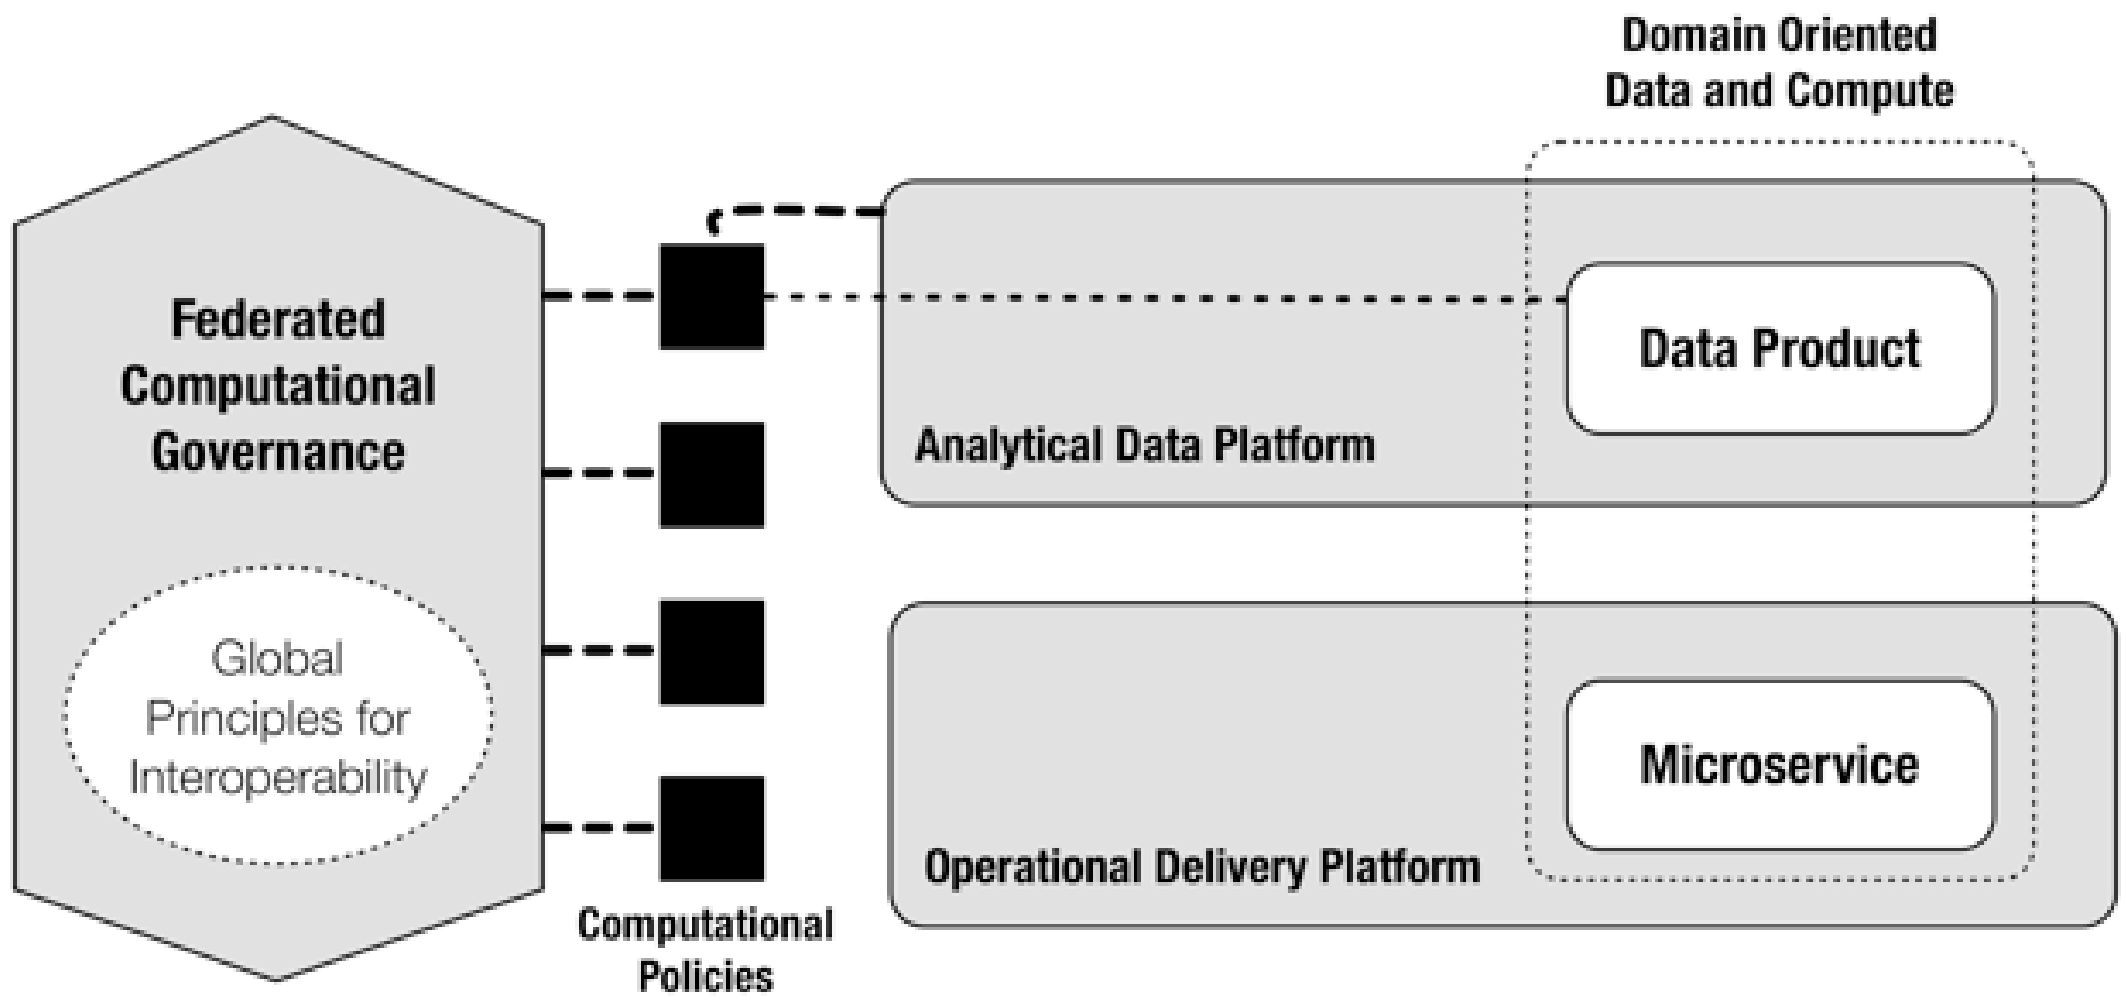
\includegraphics[width=11cm]{LogicalArchitecture.png}
		\caption{Data Mesh Logical Architecture \cite{machado2022data}}
		\label{LogicalArchitecture}
	\end{framed}
\end{figure}

\begin{xltabular}{\textwidth}{||s|m|b|}
	\caption{Data mesh logical architectural components} \label{tab:LogicArch} \\
	
	\hline \multicolumn{1}{||s|}{\textbf{Aspect}} & \multicolumn{1}{m|}{\parbox{.17\textwidth}{\textbf{Architectural component}}} & \multicolumn{1}{b|}{\textbf{Description}} \\ \hline 
	\endfirsthead
	
	\multicolumn{3}{c}%
	{\tablename\ \thetable{} \textit{-- continued from previous page}} \\
	\hline \multicolumn{1}{||s|}{\textbf{Aspect}} & \multicolumn{1}{m|}{\parbox{.17\textwidth}{\textbf{Architectural component}}} & \multicolumn{1}{b|}{\textbf{Description}} \\ \hline 
	\endhead
	
	\hline \multicolumn{3}{||r|}{{\textit{continued on next page --}}} \\ \hline
	\endfoot
	
	\hline
	\endlastfoot
	
	\multirow{3}{*}{\parbox{.13\textwidth}{\vskip 5pt Domain- Oriented  Data Sharing Interfaces}} & Domain & Systems, data products, and a cross-functional team aligned to serve a business domain function and outcomes and share its analytical and operational capabilities with the wider business and customers. \\
	\cline{2-3}
	& Domain analytical data interfaces & Standardized interfaces that discover, access, and share domain-oriented data products.\newline
	The proprietary platforms need to offer open interfaces to make data sharing more convenient and interoperable with other hosting platforms. \\
	\cline{2-3}
	& Domain operational interfaces & APIs and applications through which a business domain shares its transactional capabilities and state with the wider organization.\\
	\cline{1-3}
	\multirow{3}{*}{\parbox{.13\textwidth}{\vskip 5pt Data product quantum}} & Data product structural components & Data product implemented as an architecture quantum that encapsulates all the structural components it needs to do its job - code, data, infrastructure specifications, and policies. \newline It is referred to in architectural discussions. It is used interchangeably with data products. \\
	\cline{2-3}
	& Data Product Data Sharing Interactions & There are many technologies for implementing a data product’s input and output data port of data mesh, but it shares the common properties:
	\begin{itemize}[nosep]
		\item \textbf{Input data port:} A data product’s mechanisms to continuously receive data from one or multiple upstream sources.
		\item \textbf{Output data port:} A data product’s standardized APIs to continuously share data. \vspace{-.3cm}
	\end{itemize} \\
	\cline{2-3}
	& Discovery and observability APIs & A data product’s standard APIs to provide discoverability information - to find, address, learn, and explore a data product - and observability information such as lineage, metrics, logs, etc.\\
	\cline{1-3}
	\multirow{4}{*}{\parbox{.13\textwidth}{The Multiplane Data Platform}} & Platform plane & A group of self-serve platform capabilities with high functional cohesion surfaced through APIs.\\
	\cline{2-3}
	& Data infrastructure (utility) plane & Platform plane providing low-level infrastructure resource management - compute, storage, identity, etc.\\
	\cline{2-3}
	& Data product experience plane & Platform plan providing operations on a data product.\\
	\cline{2-3}
	& Mesh experience & Platform plane providing operations on the mesh of connected data products.\\
	\cline{1-3}
	\multirow{4}{*}{\parbox{.13\textwidth}{Embedded Computational Policies}} & Data product container & A mechanism to bundle all the structural components of a data product, deployed and run as a single unit with its sidecar.\\
	\cline{2-3}
	& Data product sidecar & The accompanying process to the data product implements cross-functional and standardized behaviors.\\
	\cline{2-3}
	& Control port & A data product’s standard APIs to configure policies or perform highly privileged governance operations.\\
\end{xltabular}

\begin{figure}[h]
	\begin{framed}
		\centering
		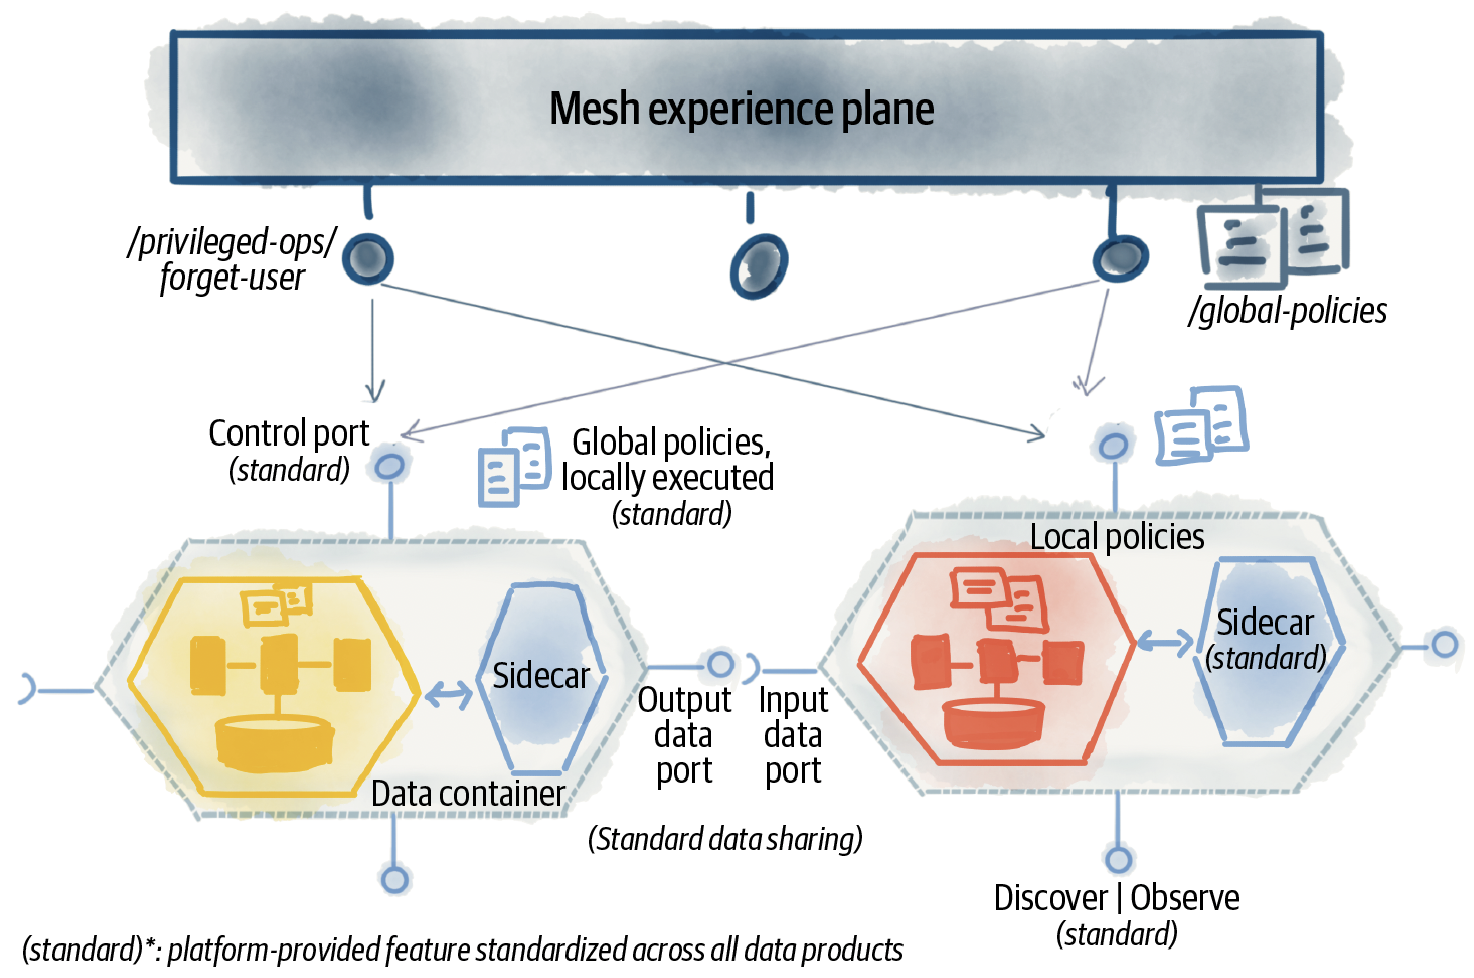
\includegraphics[width=10cm]{LogicalComponents.png}
		\caption{The logical architectural components of embedded computational policies}
		\label{LogicalComponents}
	\end{framed}
\end{figure}
\vspace{-.5cm}
It is intentionally that the technology evolves to the point that we can get the logical architecture and its physical implementation as close to each other as possible. \cite{datamesh2022p3}


\subsection{The Multiplane Data Platform Architecture}
As we have discussed previously, the multiplane data platform consists of three planes, with the interactive diagram as figure \ref{multiplane}.

\begin{figure}[h]
	\begin{framed}
		\centering
		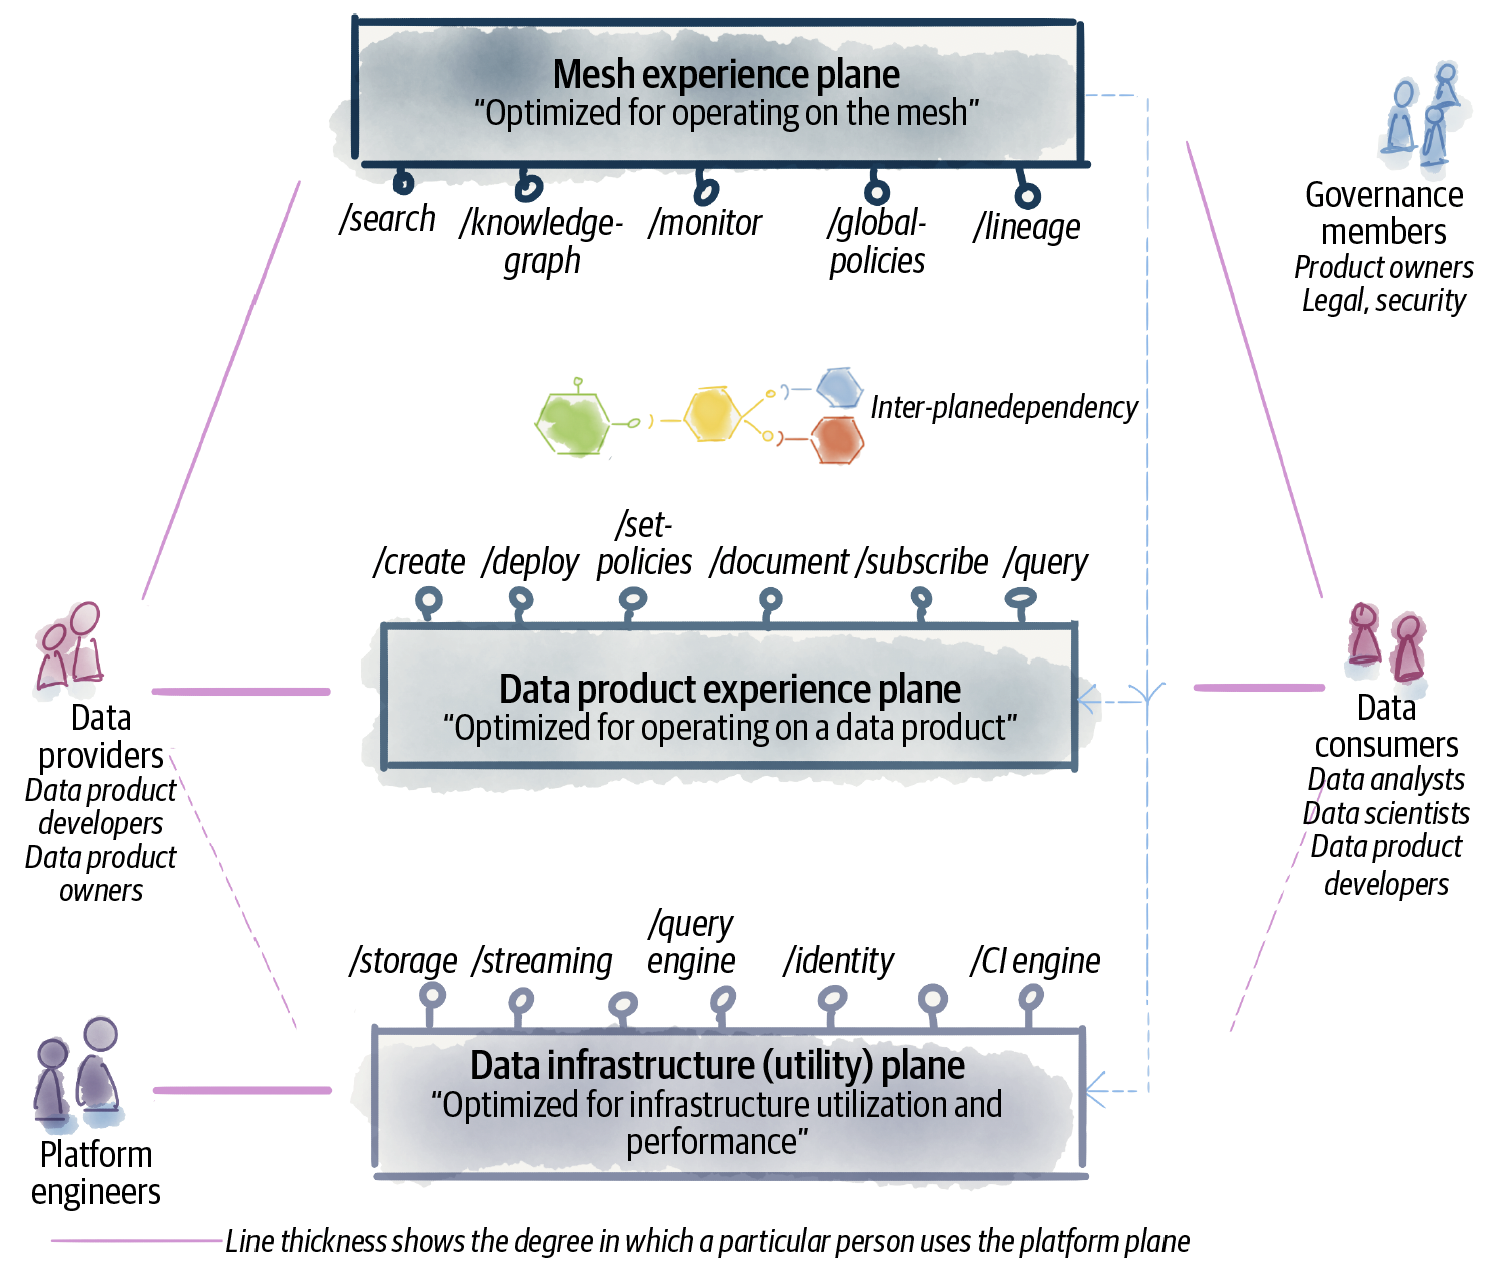
\includegraphics[width=12cm]{multiplane.png}
		\caption{Multiplane self-serve platform and platform users}
		\label{multiplane}
	\end{framed}
	\vspace{-.5cm}
\end{figure}

The data product experience plane provides operations on a data product and manages the complexity of provisioning its underlying infrastructure, while the data infrastructure utility plane optimizes the resources' performance and utilization to get the best out of the underlying infrastructure providers. The most important idea is to understand the main journeys of the platform users and evaluate how to make it easy for them to complete their journeys.
\vspace{-.3cm}
\subsubsection*{Data Product Developer Journey}
\begin{figure}[h]
	\begin{framed}
		\centering
		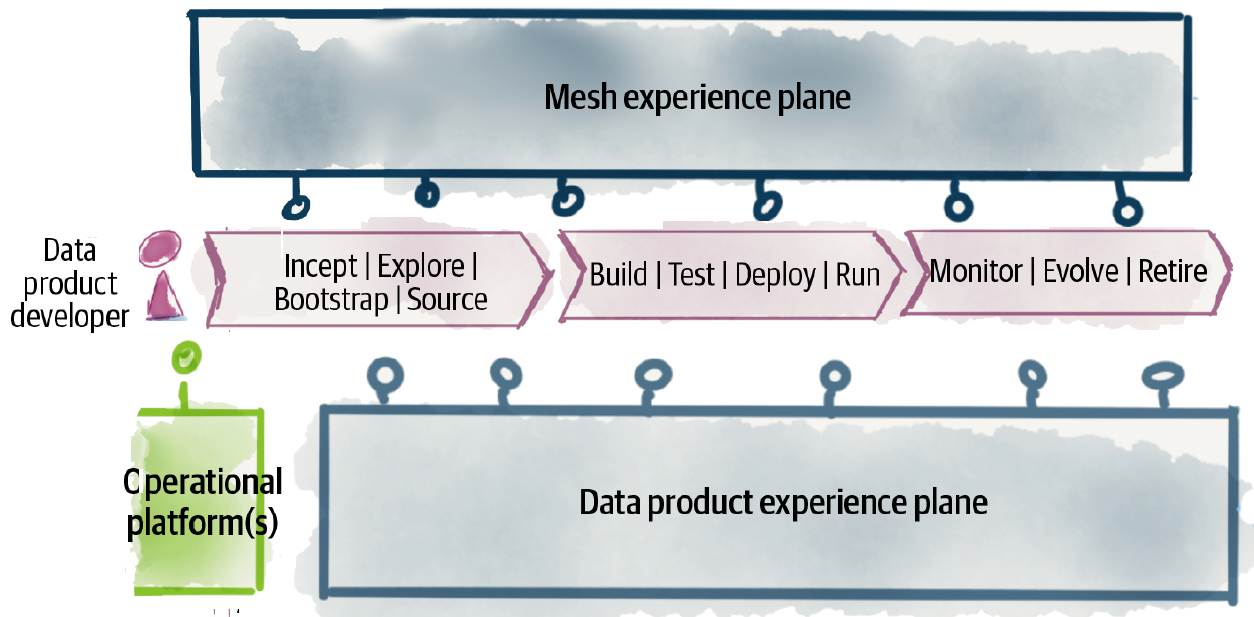
\includegraphics[width=10cm]{DataProductDevJourney.png}
		\caption{High-level example of data product development journey using the platform}
		\label{DataProductDevJourney}
	\end{framed}
\end{figure}

Creating and operating a data product is one of the most important journeys of a data product developer. This is a comprehensive and long-term obligation that adheres to the continuous delivery premise of "everyone is responsible." A data product development journey interacts with other journeys. Let’s look at the figure \ref{DataProductDevJourney} for an example of high-level stages of data product development and how the platform interfaces are designed to support them.

We should go deeper to consider each stage of the platform planes and interfaces
\begin{xltabular}{\textwidth}{||s|m|m|b|}
	\caption{Example interfaces provided by the platform planes} \label{tab:PlatformPlanes} \\
	
	\hline \multicolumn{1}{||s|}{\textbf{Phase}} & \textbf{Platform plane} & \textbf{Platform interface} &  \multicolumn{1}{b|}{\textbf{Platform interface description}}\\ \hline 
	\endfirsthead
	
	\multicolumn{4}{c}%
	{\tablename\ \thetable{} \textit{-- continued from previous page}} \\
	
	\hline \multicolumn{1}{||s|}{\textbf{Phase}} & \textbf{Platform plane} & \textbf{Platform interface} &  \multicolumn{1}{b|}{\textbf{Platform interface description}}\\ \hline  
	\endhead
	
	\hline \multicolumn{4}{||r|}{{\textit{continued on next page --}}} \\ \hline
	\endfoot
	
	\hline
	\endlastfoot
	
	\multicolumn{4}{||l|}{{\textbf{Data product inception}}} \\
	\cline{1-4} 
	\multirow{3}{*}{\parbox{.13\textwidth}{Incept |Explore}} & \multirow{3}{*}{\parbox{.13\textwidth}{Mesh experience}} & \verb*|/search| & Search existing data products based on parameters such as operational systems, domains, and types of data. \\
	\cline{3-4}
	& & \verb*|/knowledge| \verb*|-graph| & Browse the mesh of related data products’ semantic models. Traverse their semantic relationship to identify the desired sources of data. \\
	\cline{3-4}
	& & \verb*|/lineage| & Traverse the lineage of input-output data to identify desired sources based on origin and transformations. \\
	\cline{1-4}
	\multirow{6}{*}{\parbox{.13\textwidth}{Bootstrap |Source}} & \multirow{5}{*}{\parbox{.13\textwidth}{Data product experience}} & \verb*|/{dp}/| \verb*|discover| & Once a source is identified, access all the data product discoverability information such as documentation, data model, available output ports, etc. \\
	\cline{3-4}
	& & \verb*|/{dp}/| \verb*|observe|& Access data product guarantees and metrics in real-time, such as release frequency, last release date, and data quality metrics. \\
	\cline{3-4}
	& & \verb*|/init| & API bootstraps a barebones data product with infrastructure to connect to sources, access data, run transformations, and serve output in a single access mode. \\
	\cline{3-4}
	& & \verb*|/connect| & The data product gets access to the source by connecting to it, validating access control policies and triggering a request for permission. \\ \cline{3-4}
	& & \verb*|/{dp}/| \verb*|{output}/| \verb*|query| \verb*|/{dp}/| \verb*|{output}/| \verb*|subscribe| & Read data from a particular output port of the source data product, either in a pull-based querying model or subscribing to changes. \\
	\cline{2-4}
	& Mesh experience & \verb*|/register| & Data products are registered with the mesh and given a unique global identifier and address, making them visible to the governance process. \\
	\cline{1-4}
	
	\multicolumn{4}{||l|}{{\textbf{Data product development}}} \\
	\cline{1-4}
	Build & \multirow{5}{*}{\parbox{.13\textwidth}{Data product experience}} & \verb*|/build| & Compile, validate, and compose components of a data product into a deployable artifact. \newline See Table \ref{tab:PlatformPlanes} for the data infrastructure plane interfaces used during this phase. \\
	\cline{1-1}\cline{3-4}
	Test & & \verb*|/test|& Testing capabilities are offered in different deployment environments to test various aspects of a data product, such as data transformation, integrity, versioning, data profile, and bias. \\
	\cline{1-1}\cline{3-4}
	Deploy & & \verb*|/deploy| & Deploy a data product to multiple environments, including local, development, pre-production, and production.\\
	\cline{1-1}\cline{3-4}
	Run & & \verb*|/start| \verb*|/stop| & Run or stop running the data product instance in a particular environment. \\
	\cline{1-1}\cline{3-4}
	Build/ Test/ Deploy/ Run & & \verb*|/local-| \verb*|policies| & The platform facilitates configuration and authoring of these policies locally, during the development of a data product, their validation during test, and their execution during access to data. \\
	\cline{1-4}
	Build/ Test/ Deploy/ Run & Mesh experience & \verb*|/global-| \verb*|policies| & The platform enables authoring of the global policies and application of these policies by all data products. \\
	\cline{1-4}
	
	\multicolumn{4}{||l|}{{\textbf{Data product maintenance}}} \\
	\cline{1-4} 
	
	& \multirow{6}{*}{\parbox{.13\textwidth}{Data product experience}} & \verb*|/{dp}/status| & Checking the status of a data product. \\
	\cline{3-4}
	Maintain, Evolve, and Retire & & \verb*|/{dp}/logs| \verb*|/{dp}/traces| \verb*|/{dp}/| \verb*|metrics| & Data products emit runtime observability information such as logs, traces, and metrics to be used by mesh layer monitoring services. \\
	\cline{3-4}
	& & \verb*|/{dp}/| \verb*|accesses| & The logs of all accesses to the data product. \\
	\cline{3-4}
	& & \verb*|/{dp}/cost| & Tracking the operational cost of a data product. This can be calculated based on the resource allocation and usage. \\
	\cline{3-4}
	& & \verb*|/migrate| & Updating a data product revision is a simple process of build and deploy. \\
	\cline{3-4}
	& & \verb*|/{dp}/| \verb*|controls| & Data products are registered with a unique global identifier and address, making them visible to governance. \\
	\cline{2-4}
	& \multirow{3}{*}{\parbox{.13\textwidth}{Mesh experience}}& \verb*|/monitor| & Multiple monitoring abilities at the mesh level, logs, status, compliance, etc. \\
	\cline{3-4}
	& & \verb*|/notificat| \verb*|ions|& Notification and alerting in response to detected anomalies of the mesh. \\
	\cline{3-4}
	& & \verb*|/global-| \verb*|controls| & High-privilege administrative controls can be invoked on data products. \\
\end{xltabular}
\vspace{-.3cm}
The data infrastructure plane is a key enabler in lowering the cost and effort required to code or configure components of a data product. Developers interact with the data product experience plane to build, deploy, and test a single data quantum. The data product experience plane delegates the implementation of the data product components to the data infrastructure plane.

\begin{figure}[h]
	\begin{framed}
		\centering
		\vspace*{-.3cm}
		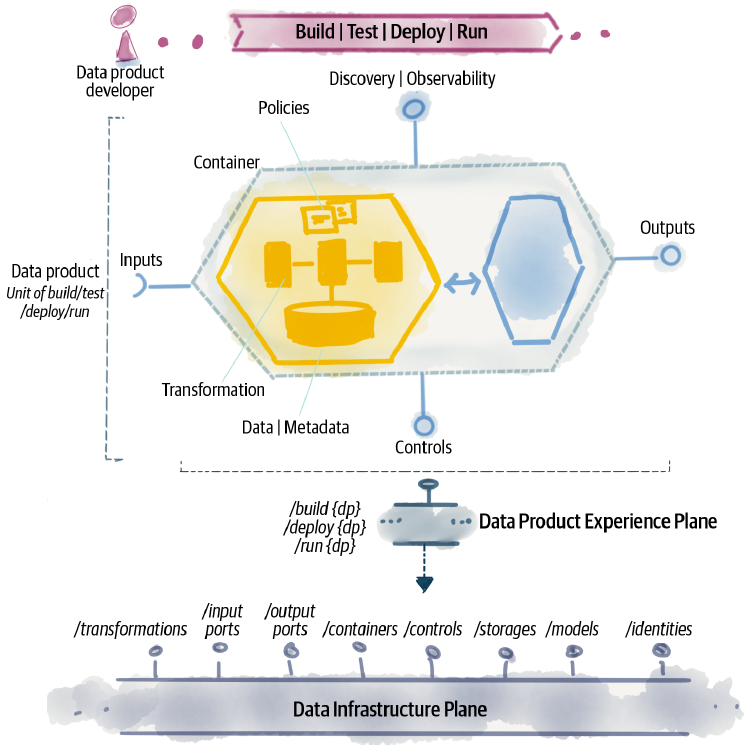
\includegraphics[width=10.5cm]{DataInfras.png}
		\caption{Example of data infrastructure plane to support data product delivery}
		\label{DataInfras}
	\end{framed}
\end{figure}


\begin{xltabular}{\textwidth}{||m|m|b|}
	\caption{Data platform interfaces that support data product experience plane APIs} \label{tab:InfrasPlanes} \\
	
	\hline \textbf{Platform plane} & \textbf{Platform interface} &  \multicolumn{1}{b|}{\textbf{Platform interface description}}\\ \hline 
	\endfirsthead
	
	\multicolumn{3}{c}%
	{\tablename\ \thetable{} \textit{-- continued from previous page}} \\
	
	\hline \textbf{Platform plane} & \textbf{Platform interface} &  \multicolumn{1}{b|}{\textbf{Platform interface description}}\\ \hline  
	\endhead
	
	\hline \multicolumn{3}{||r|}{{\textit{continued on next page --}}} \\ \hline
	\endfoot
	
	\hline
	\endlastfoot

	\multirow{5}{*}{\parbox{.13\textwidth}{Data product experience}} & \verb*|/{dp}/logs| \verb*|/{dp}/traces| \verb*|/{dp}/metrics| & Data products emit runtime observability information such as logs, traces, and metrics to be used by mesh layer monitoring services. \\
	\cline{2-3}
	& \verb*|/{dp}/status| & Checking the status of a data product. \\
	\cline{2-3}
	& \verb*|/{dp}/accesses| & The logs of all accesses to the data product. \\
	\cline{2-3}
	& \verb*|/{dp}/cost| & Tracking the operational cost of a data product. This can be calculated based on the resource allocation and usage. \\
	\cline{2-3}
	& \verb*|/migrate| & Ability to migrate a data product to a new environment. Updating the data product revision is simply a function of build and deploy. \\
	\cline{1-3}
	\multirow{3}{*}{\parbox{.13\textwidth}{Mesh experience}}& \verb*|/monitor| & Multiple monitoring abilities at the mesh level, logs, status, compliance, etc. \\
	\cline{2-3}
	& \verb*|/notifications|& Notification and alerting in response to detected anomalies of the mesh. \\
	\cline{2-3}
	& \verb*|/global-| \verb*|controls| & Ability to invoke high-privileged administrative controls such as right to be forgotten on a collection of data products on the mesh. \\
	\cline{1-3}
	Data product experience plane & \verb*|/{dp}/controls| & Data products are registered with the mesh and given a unique global identifier and address, making them visible to the governance process. \\
\end{xltabular}

\subsubsection*{Data Product Consumer Journey}
A data consumer is a user with various skills and responsibilities, such as consuming existing data products to train an ML model and then deploying it as a data product. ML models can be deployed as a microservice or as the transformation logic of a data product.

The data scientist's journey to continuously deliver an ML model as a data product follows the practice of continuous delivery for ML (CD4ML\footnote{This process is also known as MLOps; however, I use the CD4ML notation since it overlays and integrates closely with continuous delivery of software and data products.}) to continuously hypothesize, train, deploy, monitor, and improve the model in rapid feedback loops. The figure \ref{MLJourney} illustrate this journey.

\begin{figure}[h]
	\vspace*{-.3cm}
	\begin{framed}
		\centering
		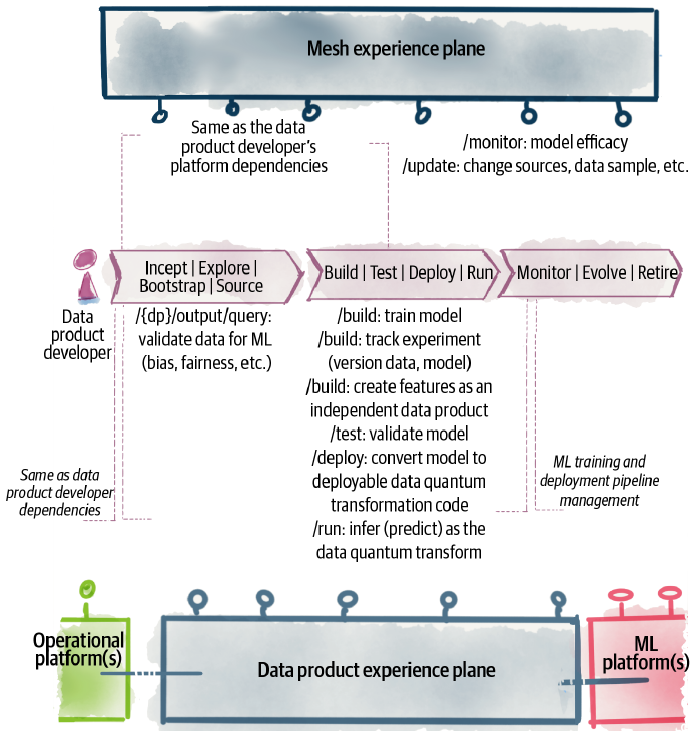
\includegraphics[width=10.5cm]{MLJourney.png}
		\caption{Example of ML model development journey}
		\label{MLJourney}
	\end{framed}
\end{figure}

In conclusion, there is no single entity such as a platform but rather a set of well-integrated services, such as APIs, SDKs, and libraries that provide a seamless experience for users. Additionally, the separation of planes should be respected to optimize both for the human experience and machine efficiency.

\let\cleardoublepage\clearpage
\chapter{Data Product Design \& Implementation}
\section{What is Data Product and Its Canvas}
Data product is a core component in data mesh architecture. Conceptually, a mesh is a graph, or network, composed of nodes and connecting edges. Each node in a data mesh is referred to as a data product. Every data product resides within a confined context, and a single bounded context may contain multiple data products.

Data product can be everything that has value for consumers (e.g., a database table, raw unstructured files, dashboard, data stream, etc.). It contains all data, code, and interfaces to serve analytical data needs. Data product connects to sources, such as operational systems or other data products and perform data transformation. It serves data sets in one or many output ports. \cite{datameshweb}

\begin{figure}[h]
	\vspace*{-.3cm}
	\begin{framed}
		\centering
		
\includegraphics[width=10.5cm]{boring.jpg}
		\caption{Data Product Simple Canvas}
		\label{DPCanvas}
	\end{framed}
\end{figure}

A Data Product Canvas is a visual framework that guides a team through the data product specification. In total, the canvas consists of ten building blocks:
	\begin{itemize}[nosep]
		\item \textbf{Domain:} Data products should belong to one domain team, with accountability, requirements, questions, and fixes.
		\item \textbf{Data Product Name:} This should follow a common naming strategy.
		\item \textbf{Consumer and Use Case:} Data product design follows "Product Thinking" to identify consumer needs.
		\item \textbf{Output Port:} Output ports define the format and consumption protocol for data.
		\item \textbf{Metadata:} This includes data product ownership, schema, semantics, security.
		\item \textbf{Input Ports:} Input ports define data format and protocol for reading.
		\item \textbf{Data Product Design:} Design a data product on a conceptual level by specifying data ingestion, storage, transport, etc.
		\item \textbf{Observability:} This includes quality, operational metrics, and service level objectives to build trustworthiness in data products.
		\item \textbf{Ubiquitous Language:} Common language shared for operational systems and data products.
		\item \textbf{Classification:} Classifying data as source-aligned, aggregated, or consumer-aligned.
	\end{itemize}


\section{Design a Data Product by Affordances}
Data mesh is a distributed scale-out architecture that designs data products as self-contained, autonomous, and coequal nodes, providing users and developers with the capabilities they need to do their job: discover, understand, use, build, govern, and debug.

In addition to four common constituents of architecture\footnote{Structure, Characteristics, Decisions, Principles}, we introduce and focus on designing a data product by another element: affordances \cite{norman2002design}.

Table \ref{tab:affordances} lists affordances for a data product to autonomously transform and serve meaningful, understandable, trustworthy data that can be connected to other data in the ecosystem. It has all the structural components to do its job, and its dependencies to other data products or platform services are through APIs with explicit contracts, creating loose coupling.

\begin{xltabular}{\textwidth}{||s|b|}
	\caption{Data product affordances} \label{tab:affordances} \\
	
	\hline \textbf{Affordances} & \multicolumn{1}{b|}{\textbf{Description}}\\ \hline 
	\endfirsthead
	
	\multicolumn{2}{c}%
	{\tablename\ \thetable{} \textit{-- continued from previous page}} \\
	
	\hline \textbf{Affordances} & \multicolumn{1}{b|}{\textbf{Description}}\\ \hline 
	\endhead
	
	\hline \multicolumn{2}{||r|}{{\textit{continued on next page --}}} \\ \hline
	\endfoot
	
	\hline
	\endlastfoot
	
	
	Serve Data & The data product shares immutable and bitemporal data, allowing users to access it for multiple purposes, but not for transactional and operational applications. \\
	\cline{1-2}
	Consume Data & The data product consumes data from upstream sources, but only from sources it identifies and configures through the platform, not from sources it does not identify and configure. \\
	\cline{1-2}
	Transform Data & The data product transforms input data into new data, which can be program code, a machine learning model, or a complex query. It can generate new data or improve the quality of input data. \\
	\cline{1-2}
	Discover | Understand |Explore | Trust & The data product serves APIs and information that affords data product users to discover, explore, understand, and trust it. \\
	\cline{1-2}
	Compose Data & The data product allows users to compose, correlate, and join data with other data products, while the data quantum provides programmatic data composability by performing set operations. \\
	\cline{1-2}
	Manage Life Cycle & Data products provide a set of configuration and code to enable developers to build, provision, and maintain them. \\
	\cline{1-2}
	Observe | Debug | Audit & The data product provides programmatic APIs to enable users to monitor its behavior, debug issues, and audit it. \\
	\cline{1-2}
	Govern & The data product provides data users and the mesh experience plane with APIs and policies to self-govern their data, enabling build-time configuration and runtime execution of policies. It also maintains data security and protects privacy and confidentiality through encryption. \\
\end{xltabular}

Data products must be designed to meet the data mesh objective of "getting value from data at scale", that means, we have to satisfy:
	\begin{itemize}[nosep]
		\item Design for change: Design for change is essential for data products to respond gracefully to change, such as fronting aspects with APIs or adding time.
		\item Design for scale: A data product must scale out while maintaining agility and speed of access.
		\item Design for value: Data product interfaces should focus on sharing easily understandable, trustworthy data with minimal friction.
	\end{itemize}

The final thing is design simple and local rules and behaviors in data products to create mesh-level knowledge and intelligence.

\section{Consuming, Transforming \& Serving Data}
A data product’s primary job is to consume data from upstream sources using its input data ports, transform it, and serve the result as permanently accessible data via its output data ports.

\subsection{Serve data}
Data products serve domain-oriented data to diverse consumers through output data ports and APIs. Serve data design has some properties:
	\begin{itemize}[nosep]
		\item Multimodal data: Data products serve data of a domain with a specific and unique domain semantic. They can be served in different formats. When a user accesses a data product, they first learn about its semantic and then access one of its output APIs.
		\item Immutable data: Immutable data is a key axiom in functional programming. This is relevant to analytical use cases, as it allows users to rerun analytics in a repeatable way.
		\item Bitemporal data: Bitemporal data modeling records two timestamps: actual time and processing time, making it possible to serve data as immutable entities and perform temporal analysis and time travel.
	\end{itemize}

\begin{figure}
	\begin{framed}
		\centering
		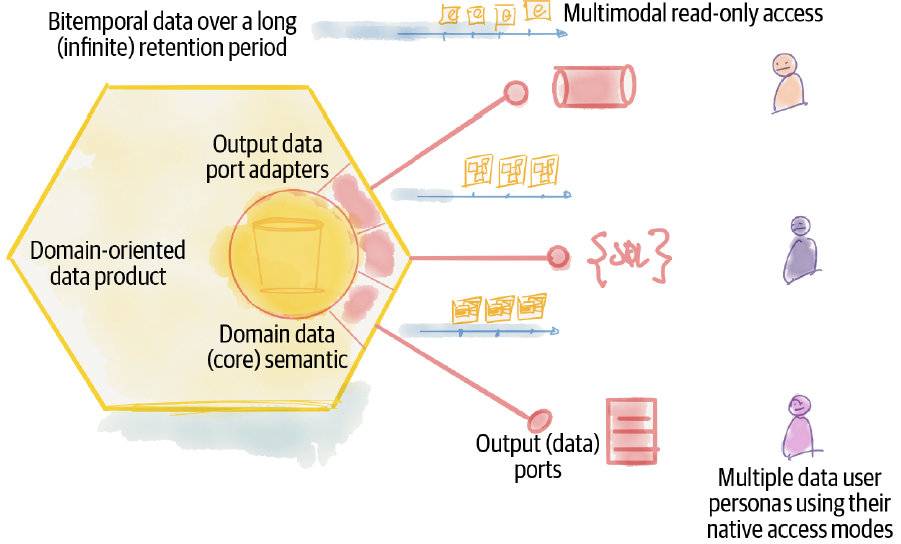
\includegraphics[width=10.5cm]{ServeData.png}
		\caption{Data product’s high-level components to design serve data}
		\label{ServeData}
	\end{framed}
\end{figure}

\begin{xltabular}{\textwidth}{||s|b|}
	\caption{High-level data product components to serve data} \label{tab:servedata} \\
	
	\hline \textbf{Component} & \multicolumn{1}{b|}{\textbf{Description}}\\ \hline 
	\endfirsthead
	
	\multicolumn{2}{c}%
	{\tablename\ \thetable{} \textit{-- continued from previous page}} \\
	
	\hline \textbf{Component} & \multicolumn{1}{b|}{\textbf{Description}}\\ \hline 
	\endhead
	
	\hline \multicolumn{2}{||r|}{{\textit{continued on next page --}}} \\ \hline
	\endfoot
	
	\hline
	\endlastfoot
	
	Output data port & APIs are used to serve data according to a specific mode of access for a particular spatial format. \\
	\cline{1-2}
	Output (data) port adapter & The code responsible for presenting data for a particular output port is either a step in the data product's transformation code or a runtime gateway. \\
	\cline{1-2}
	Core data semantic & Expression of the data semantic - agnostic to the modes of access or its spatial syntax. \\
\end{xltabular}

\subsection{Consume Data}
In most of cases, data in organizations originates from internal or external systems, and data products consume it from one or multiple sources. Input data ports are a logical architectural construct that allow a data product to connect to a source, execute queries, and receive data as a continuous stream or one-off payload. Consume data design has some notable characteristics that impact the design of a data product’s input data:

\begin{itemize}[nosep]
	\item Archetypes of data sources: collaborate operational systems, data products or itself.
	\item Locality of Data Consumption.
\end{itemize}

\begin{xltabular}{\textwidth}{||s|b|}
	\caption{High-level components to design consume data} \label{tab:consumedata} \\
	
	\hline \textbf{Component} & \multicolumn{1}{b|}{\textbf{Description}}\\ \hline 
	\endfirsthead
	
	\multicolumn{2}{c}%
	{\tablename\ \thetable{} \textit{-- continued from previous page}} \\
	
	\hline \textbf{Component} & \multicolumn{1}{b|}{\textbf{Description}}\\ \hline 
	\endhead
	
	\hline \multicolumn{2}{||r|}{{\textit{continued on next page --}}} \\ \hline
	\endfoot
	
	\hline
	\endlastfoot
	
	Input data port & The mechanism by which a data product receives its source data and makes it available for internal transformation. \\
	\cline{1-2}
	Input data port specification & A declarative specification of input data ports that configures from where and how data is consumed. \\
	\cline{1-2}
	Asynchronous input data port & Asynchronous input ports reactively execute transformation code when necessary source data is available. \\
	\cline{1-2}
	Remote query & An input port specification can include a query executed on the source to receive desired data, reducing the amount of data fetched redundantly. \\
	\cline{1-2}
	Input port synchronizer and temporary storage & Temporary storage is necessary to keep track of observed and unprocessed data until all observations are available for processing. \\
\end{xltabular}

\begin{figure}[h]
	\begin{framed}
			\centering
			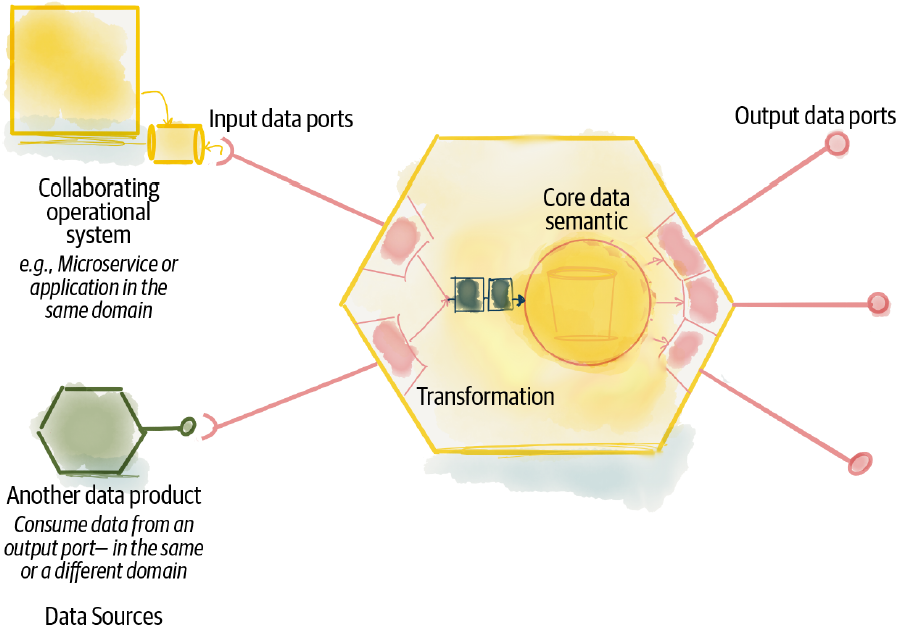
\includegraphics[width=10.5cm]{ConsumeData.png}
			\caption{Data product’s design to consume data}
			\label{ConsumeData}
		\end{framed}
\end{figure}

\subsection{Transform Data}
Data products are created to share a new analytical model of existing data. Transformation is an internal implementation of a data product and is controlled by it. It is up to the data product developer to choose how to implement the transformation, and it is helpful to look at a few different ways of implementation:
	\begin{itemize}[nosep]
		\item Nonprogrammatic: Nonprogrammatic transformations use relational algebra or flow-based functions to capture the intent of how data is transformed, but are limited to the features of the statement.
		\item Programmatic: Programmatic data processing uses code logic, conditions, and statements to transform data, allowing it to be modularized and tested, making it more extensible.
		\item Dataflow-Based: Dataflow programming is a natural paradigm for implementing transformation code, as long as the pipeline stages don't extend beyond the boundary of a data product.
		\item ML Model: ML models can be deployed in many contexts to make predictions and store recommendations for playlist extension.
		\item Time-Variant: Transformations respect the axes of time, processing and actual, by keeping track of processing time and generating output with actual time.
	\end{itemize}

\begin{figure}[h]
	\begin{framed}
		\centering
		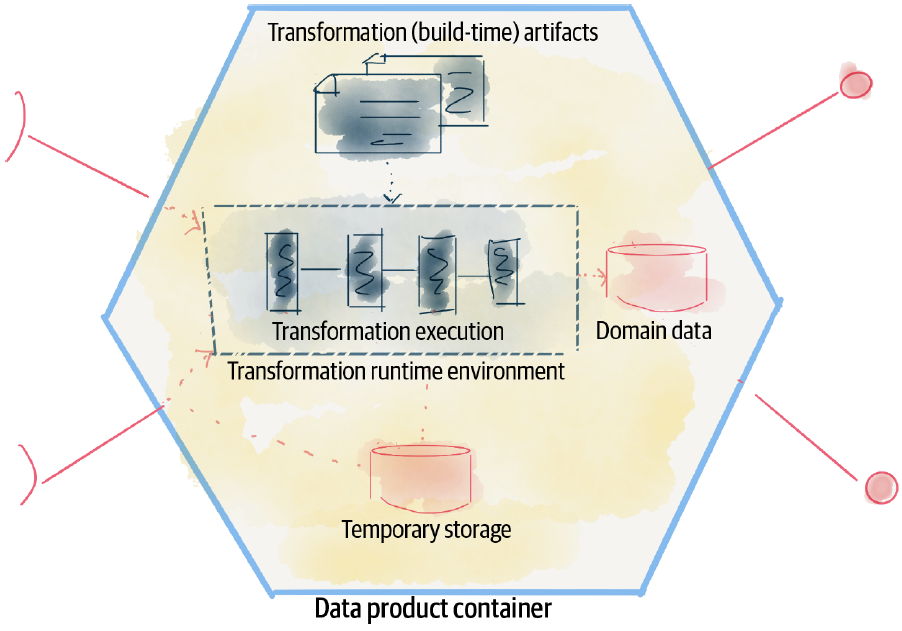
\includegraphics[width=10.5cm]{TransformData.png}
		\caption{High-level components to design transformation for data products}
		\label{TransformData}
	\end{framed}
\end{figure}

\begin{xltabular}{\textwidth}{||s|b|}
	\caption{High-level components to transform data for a data product} \label{tab:transformdata} \\
	
	\hline \textbf{Component} & \multicolumn{1}{b|}{\textbf{Description}}\\ \hline 
	\endfirsthead
	
	\multicolumn{2}{c}%
	{\tablename\ \thetable{} \textit{-- continued from previous page}} \\
	
	\hline \textbf{Component} & \multicolumn{1}{b|}{\textbf{Description}}\\ \hline 
	\endhead
	
	\hline \multicolumn{2}{||r|}{{\textit{continued on next page --}}} \\ \hline
	\endfoot
	
	\hline
	\endlastfoot
	
	Transformation artifact(s) & Code, configuration, statement, or model executes transformation on input data. \\
	\cline{1-2}
	Transformation runtime environment & Transformations require a computational environment to execute, provided by the underlying platform. \\
	\cline{1-2}
	Temporary storage & Platform provides temporary storage for transformation code steps. \\
\end{xltabular}

\section{Discovering, Understanding \& Composing Data}
\subsection{Discover, Understand, Trust, and Explore}
Data products are responsible for bridging the gap between the known and unknown, so users trust them. Interfaces and behaviors are designed to share information about data semantics, formats, usage documentations, statistical properties, expected quality, timeliness, and other metrics. ML-based discovery functions can be built to search, browse, examine, and get meaning from the mesh of connected data products.

To satisfy the above design, we need to follow these steps:
	\begin{enumerate}
		\item Begin discovery with self-registration,
		\item Discover the global URI,
		\item Understand semantic and syntax models,
		\item Establish trust with data guarantees,
		\item Learn with documentation.
	\end{enumerate}

The data product sidecar is a platform-provided agent that runs within the computational context of a data quantum and is responsible for cross-cutting concerns that need to be standardized across all data products. Figure demonstrates the data product sidecar’s interactions in support of discoverability. 

\begin{figure}[h]
	\begin{framed}
		\centering
		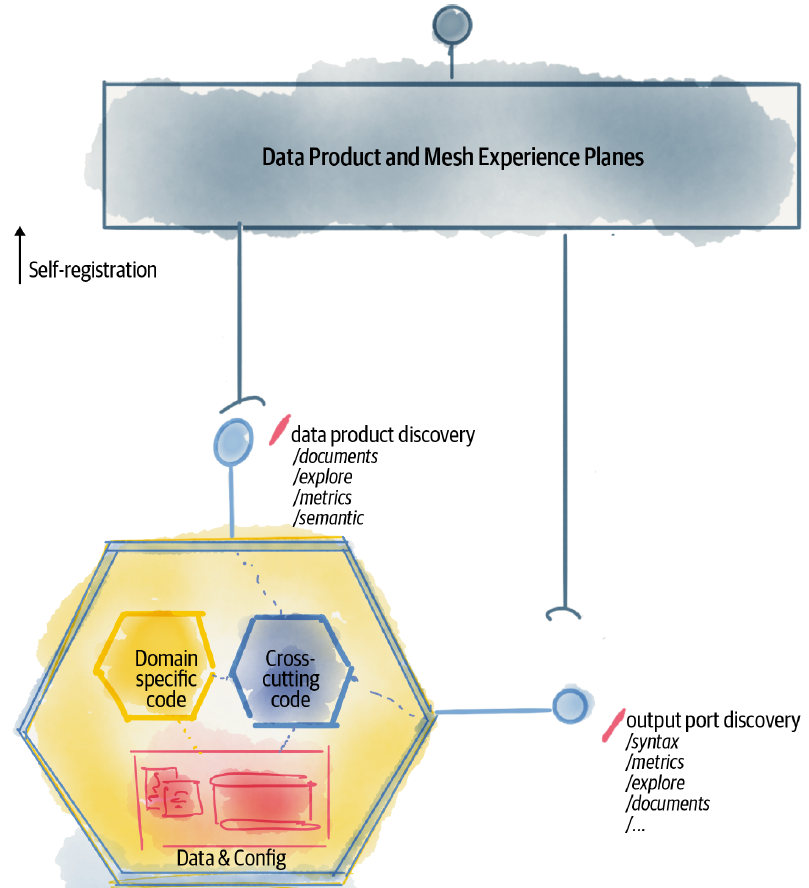
\includegraphics[width=10.5cm]{DiscoverData.png}
		\caption{A data product sidecar provides a unified model of discoverability for all data products}
		\label{DiscoverData}
	\end{framed}
\end{figure}
\vspace{-.3cm}
\subsection{Compose Data}
The design considerations for a system of distributed data models that enables data composability and quick evolution without building tightly connected or centralized models are the most essential details in this article. Ownership of a time-variant, sharable, and referenceable semantic data model, semantic model linking, a global identification system to map data across data products, and the responsibility of data product owners to continuously look for opportunities to discover and create meaningful relationships with other data products are among the design considerations. These design principles are required for individual data products to generate higher-order intelligence and understanding.

The design prioritizes loose coupling between data products and minimizing centralized synchronization points. Data composability across the mesh is based on a distributed type system (schemas) where each data product owns and controls its own life cycle.

\begin{figure}
	\begin{framed}
		\centering
		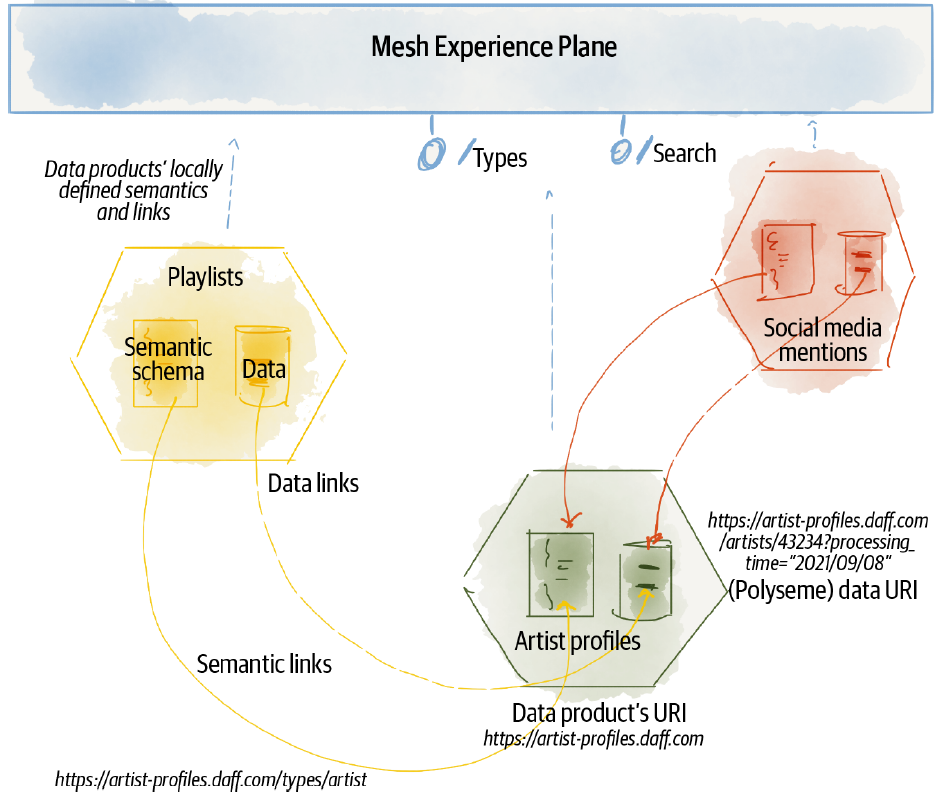
\includegraphics[width=10.5cm]{ComposeData.png}
		\caption{Data product’s high-level components to design data composability}
		\label{ComposeData}
	\end{framed}
\end{figure}

\section{Managing, Governing \& Observing Data}
\subsection{Manage the Life Cycle}
A data product's manifest is the specification of its target state, which can change and evolve during its lifetime. Developers create two groups of artifacts: source artifacts and data quantum manifest, which are used to generate the build and runtime artifacts, provision necessary resources, and run the data product container. The declarative modeling of a data product hides complexity, allowing developers to communicate various facets and properties of a data product in a standard fashion.

\begin{figure}
	\begin{framed}
		\centering
		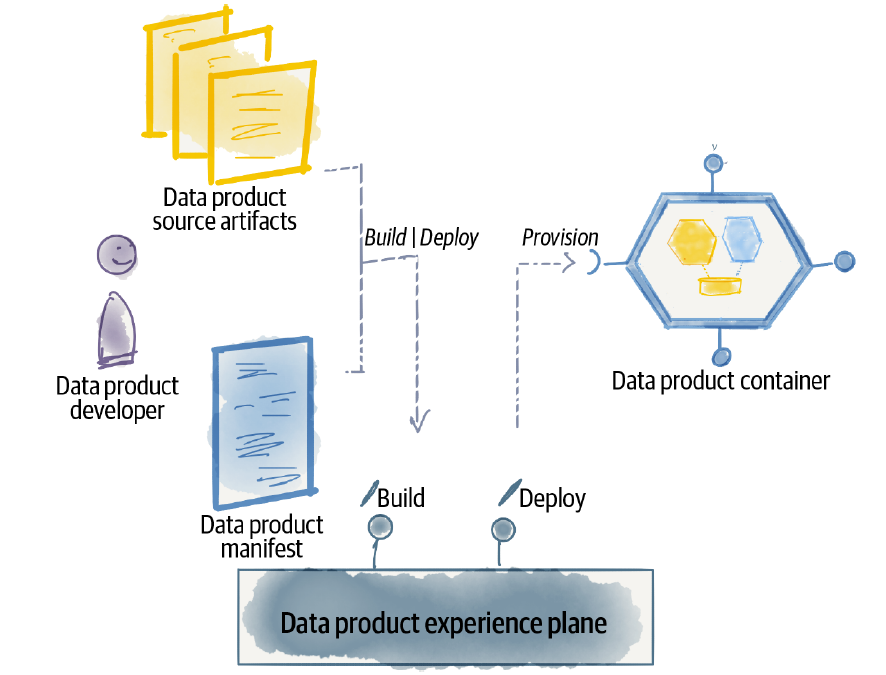
\includegraphics[width=10.5cm]{ManageLifeCycle.png}
		\caption{High-level interactions to manage the life cycle of a data product}
		\label{ManageLifeCycle}
	\end{framed}
\end{figure}

\begin{xltabular}{\textwidth}{||s|b|}
	\caption{High-level components to transform data for a data product} \label{tab:DataManifest} \\
	
	\hline \textbf{Component} & \multicolumn{1}{b|}{\textbf{Description}}\\ \hline 
	\endfirsthead
	
	\multicolumn{2}{c}%
	{\tablename\ \thetable{} \textit{-- continued from previous page}} \\
	
	\hline \textbf{Component} & \multicolumn{1}{b|}{\textbf{Description}}\\ \hline 
	\endhead
	
	\hline \multicolumn{2}{||r|}{{\textit{continued on next page --}}} \\ \hline
	\endfoot
	
	\hline
	\endlastfoot
	
	Data product’s URI & Data product’s globally unique identifier. \\
	\cline{1-2}
	Output ports & Platform declares output ports, access modes, and guarantees. \\
	\cline{1-2}
	Output port SLOs & Ports must declare the service level agreements they guarantee. \\
	\cline{1-2}
	Input ports & Declaration of input ports, data sources, and retrieval methods. \\
	\cline{1-2}
	Local policies & Configuration of local policies such as locality, confidentiality, etc. \\
	\cline{1-2}
	Source artifacts & Data product includes transformation code and input ports queries. \\
\end{xltabular}

\subsection{Govern Data}
Data products are architectural components that enable configuration and execution of policies. These components include a control port, data product sidecar, and data product container. These components work in collaboration with the mesh experience plane, which provides capabilities for governance processes such as configuring policies and the right to be forgotten globally across the mesh. Governance of policies requires observability of their state of adoption, which can be domain-specific or agnostic. Successful implementation of data mesh governance requires design characteristics such as conformance to HIPAA and guaranteed data accuracy levels.

\begin{figure}
	\begin{framed}
		\centering
		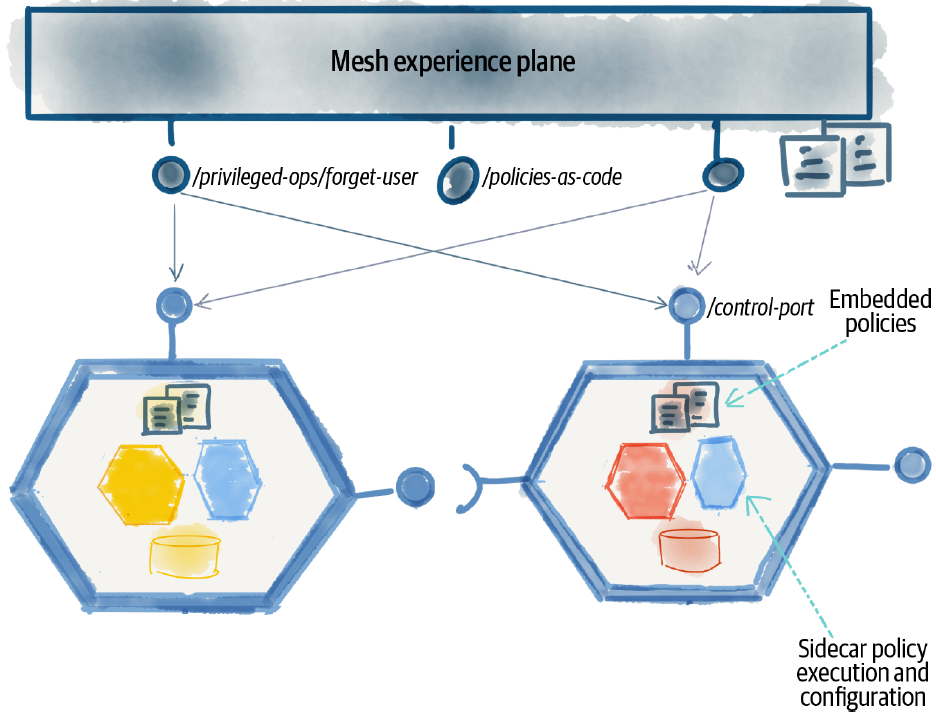
\includegraphics[width=10.5cm]{GovernData.png}
		\caption{High-level design of embedded policies as code}
		\label{GovernData}
	\end{framed}
\end{figure}

\subsection{Observe, Debug, and Audit}
Data product observability is the ability to infer the internal state of data products by observing their external outputs. The distributed architecture of data mesh creates complexity in observability, as there are many moving parts that can fail and failures may go unnoticed.

The use cases for data product observability can be summarized as follows:
	\begin{itemize}[nosep]
		\item Monitor the operational health of the mesh,
		\item Debug and perform postmortem analysis,
		\item Perform audits,
		\item Understand data lineage.
	\end{itemize}

Data mesh observability begins with each data product sharing its external output and reporting its status, allowing the experience plane to observe and monitor the mesh-level status. Some notable design characteristics of data products enable observability:
	\begin{itemize}[nosep]
		\item Observable outputs: Distributed architectures use logs, traces, and metrics to enable observability.
		\item Traceability across operational and data planes: Observability of data must extend beyond data products to operational systems to provide a complete picture of data lineage and root cause analysis.
		\item Structured and standardized observability data: Data product metrics, logs, and traces must be structured and standardized to create higher-order intelligence and insights.
		\item Domain-oriented observability data: Domain-oriented design can scale and extend observability by creating domains of observability and managing them as data products.
	\end{itemize}

\let\cleardoublepage\clearpage
%------ NOT IN THE BOOK ------
\chapter{Data Mesh in use}
%\section{Data Mesh in combination with Data Lakehouse}

\section{Frameworks and technologies for Data Mesh}
Data mesh is primarily an organizational approach, and that's why you can't buy a data mesh from a vendor. Technology, however, is important still as it acts as an enabler for data mesh, and only useful and easy to use solutions will lead to domain teams' acceptance. There are some tools for installing data mesh, such as Google Cloud Platform, AWS Platform and Data Build Tool (dbt) with Snowflake. \cite{datameshweb}

I have created a small comparison between these tools for an easy comprehension between them.

\begin{xltabular}{\textwidth}{||m|m|m|}
	\caption{Comparison between tools for data mesh} \label{tab:comparetools} \\
	
	\hline \textbf{Google Cloud Platform} & \textbf{AWS Platform} & \textbf{dbt \& Snowflake}\\ \hline 
	\endfirsthead
	
	\multicolumn{3}{c}%
	{\tablename\ \thetable{} \textit{-- continued from previous page}} \\
	
	\hline \textbf{Google Cloud Platform} & \textbf{AWS Platform} & \textbf{dbt \& Snowflake}\\ \hline 
	\endhead
	
	\hline \multicolumn{3}{||r|}{{\textit{continued on next page --}}} \\ \hline
	\endfoot
	
	\hline
	\endlastfoot
	
	Use BigQuery, Dataplex, etc. & Use AWS S3 and AWS Athena. & Use dbt and Snowflake warehouse, stage, etc. \\
	\hline
	A common infrastructure, highly integrated platform, at least for analytical data. & The primary means to share and query data products. & dbt is the default framework to engineer analytical data, Snowflake is a data warehouse. \\
	\hline
	Every domain team typically gets their own GCP project under an organization resource. & Every domain team typically has their own AWS S3 buckets to store their own data products. & Every domain team manages their own dbt projects and CI pipelines to run the models. \\
\end{xltabular}

Here, for the purpose of an enterprise, I will focus on implementing data mesh using Google Cloud Platform with supports from Apache Kafka, PostgreSQL, and Apache Airflow extension.

\begin{figure}[h]
	\begin{framed}
		\centering
		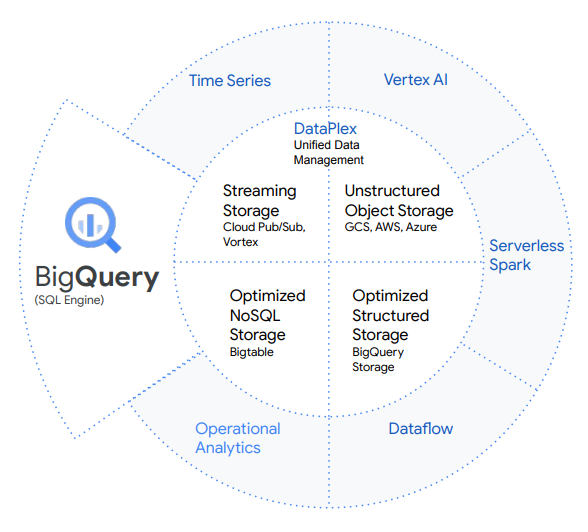
\includegraphics[width=10cm]{GCPDataMesh.png}
		\caption{Google Cloud Platform supports for data mesh}
		\label{GCPDataMesh}
	\end{framed}
\end{figure}



% check in Zalo and refs folder.
\section{Case study and Demo}
\subsection{Data contracts in Paypal Inc.}

\subsection{Data products in Daff Inc.}

\begingroup
\backmatter
\pagenumbering{alph}
\renewcommand\bibname{References}
\addcontentsline{toc}{chapter}{References}
\bibliographystyle{IEEEtran} % We choose the "plain" reference style
\bibliography{includes/refs} % Entries are in the refs.bib file
\endgroup

\clearpage
\end{document}
